% Anonymous or not; does not seem so...
% I think it is not anonymous as it says in the website " All submissions should clearly present the author information including the names of the authors, the affiliations and the emails."

% All papers accepted should have a maximum length of 9 pages (single-spaced, 2 column, 10 point font, and at least 1" margin on each side). Authors should use US Letter (8.5" x 11") paper size. Papers must have an abstract with a maximum of 300 words and a keyword list with no more than 6 keywords. Authors are required to submit their papers electronically in PDF format (postscript files can be converted using standard converters) to https://cmt.research.microsoft.com/SDM2014/ by 11:59 PM (PST), October 13, 2013.



%% Revised 10/03/01 to remove page numbering
%% Revised 10/19/01 to add space after run-in titles
%%         word space no longer needed after run-ins
%%         
%%         Possible spacing bug in \subsection fixed
%%
%% This is soda2e.all. This file is to be used for creating a paper
%% in the ACM/SIAM Preprint series with LaTeX2E. It consists of the following 
%% two files:
%%
%%       ltexpprt.tex ---- an example and documentation file
%%       ltexpprt.sty ---- the macro file
%%
%% To use, cut this file apart at the appropriate places.  You can run the
%% example file with the macros to get sample output.
%%
%%%%%%%%%%%%%%%%%%%%%%%%%%%%%  CUT HERE  %%%%%%%%%%%%%%%%%%%%%%%%%%%%%%%%%
%
%
%%%%%%%%%%%%%%%%%%%%%%%%%%  ltexpprt.tex  %%%%%%%%%%%%%%%%%%%%%%%%%%%%%%%%
%
% This is ltexpprt.tex, an example file for use with the SIAM LaTeX2E
% Preprint Series macros. It is designed to provide double-column output. 
% Please take the time to read the following comments, as they document
% how to use these macros. This file can be composed and printed out for
% use as sample output.

% Any comments or questions regarding these macros should be directed to:
%
%                 Donna Witzleben
%                 SIAM
%                 3600 University City Science Center
%                 Philadelphia, PA 19104-2688
%                 USA
%                 Telephone: (215) 382-9800
%                 Fax: (215) 386-7999
%                 e-mail: witzleben@siam.org


% This file is to be used as an example for style only. It should not be read
% for content.

%%%%%%%%%%%%%%% PLEASE NOTE THE FOLLOWING STYLE RESTRICTIONS %%%%%%%%%%%%%%%

%%  1. There are no new tags.  Existing LaTeX tags have been formatted to match
%%     the Preprint series style.    
%%
%%  2. You must use \cite in the text to mark your reference citations and 
%%     \bibitem in the listing of references at the end of your chapter. See
%%     the examples in the following file. If you are using BibTeX, please
%%     supply the bst file with the manuscript file.
%% 
%%  3. This macro is set up for two levels of headings (\section and 
%%     \subsection). The macro will automatically number the headings for you.
%%
%%  5. No running heads are to be used for this volume.
%% 
%%  6. Theorems, Lemmas, Definitions, etc. are to be double numbered, 
%%     indicating the section and the occurence of that element
%%     within that section. (For example, the first theorem in the second
%%     section would be numbered 2.1. The macro will 
%%     automatically do the numbering for you.
%%
%%  7. Figures, equations, and tables must be single-numbered. 
%%     Use existing LaTeX tags for these elements.
%%     Numbering will be done automatically.
%%   
%%
%%%%%%%%%%%%%%%%%%%%%%%%%%%%%%%%%%%%%%%%%%%%%%%%%%%%%%%%%%%%%%%%%%%%%%%%%%%%%%%



\documentclass[twoside,leqno,twocolumn]{article}  
\usepackage{ltexpprt} 
\usepackage[pdftex]{graphicx}
\usepackage{subfigure}
\usepackage{url}
\newcommand{\theHalgorithm}{\arabic{algorithm}}
\usepackage{algorithm}
\usepackage{algpseudocode}


\newcommand{\fix}{\marginpar{FIX}}
\newcommand{\new}{\marginpar{NEW}}
%\newtheorem{theorem}{Lemma}
\newtheorem{mydef}{Definition}

\usepackage{amsfonts,amsmath}
\newcommand{\vect}[1]{\mathbf{#1}}
\newcommand{\mat}[1]{\mathbf{#1}}
%%%%%%%%%%%Nos raccourcis

\renewcommand{\epsilon}{\varepsilon}
\newcommand{\be}{\beta}
\newcommand{\eps}{\varepsilon}
\newcommand{\rhon}{\rho}
\newcommand{\tmu}{\tilde{\mu}}
\newcommand{\hGn}{\hat{G}_n}
\newcommand{\logdel}{\log(\delta^{-1})}
\newcommand{\Ber}{Ber}
\newcommand{\K}{\mathrm{K}}

\newcommand{\A}{{\mat A}}
\newcommand{\B}{{\mat B}}
\newcommand{\E}{\mathbb{E}}
\newcommand{\F}{\mathcal{F}}
\newcommand{\Id}{{\mat{Id}}}
\newcommand{\I}{{\cal I}}
\newcommand{\J}{{\cal J}}
\newcommand{\N}{\mathbb{N}}
\newcommand{\R}{\mathbb{R}}
\newcommand{\Rknown}{{\mat R}}
\newcommand{\Q}{\mathbb{Q}}
\newcommand{\U}{{\mat U}}
\newcommand{\V}{{\mat V}}
\newcommand{\cK}{\mathcal{K}}
\newcommand{\cN}{\mathcal{N}}
\newcommand{\cX}{\mathcal{X}}
\newcommand{\cS}{\mathcal{S}}
\newcommand{\cP}{\mathcal{P}}
\newcommand{\oR}{\overline{R}}
\newcommand{\cF}{\mathcal{F}}
\renewcommand{\P}{\mathbb{P}}
\newcommand{\wh}{\widehat}
\newcommand{\vv}{{\vect v}}
\newcommand{\uu}{{\vect u}}


\DeclareMathOperator*{\argmax}{argmax}
\DeclareMathOperator*{\argmin}{argmin}
% \newcommand{\argmax}{\mathop{\mathrm{argmax}}}
% \newcommand{\argmin}{\mathop{\mathrm{argmin}}}
\newcommand{\ol}{\overline}
\DeclareMathOperator*{\MF}{Matrix Factorization}
\DeclareMathOperator*{\reg}{Reg}

\def\beglab{\begin{equation} \label}
\def\endlab{\end{equation}}
\def\beglabc{\begin{equation*} }
\def\endlabc{\end{equation*}}

%\newcommand{\it}{\textit}
%\newcommand{\bf}{\textbf}

\newcommand\ind{B}

\renewcommand{\thefootnote}{\arabic{footnote}}

\DeclareMathOperator{\cumrew}{CumRew}
\DeclareMathOperator{\cumreg}{Regret}
\newcommand{\irec}{{\cal IR}}
\newcommand{\rec}{{\cal R}}
\newcommand{\expexp}{\texttt{Explore-Exploit}}
\newcommand{\epsgreedy}{$\epsilon$-greedy}




\usepackage[usenames,dvipsnames]{xcolor}
\newcommand{\pp}[1]{\color{red}(pp) #1\color{black}}
\newcommand{\jm}[1]{{\color{TealBlue}(jm) #1\color{black}}}
\newcommand{\hai}[1]{\color{blue}(hai) #1\color{black}}

% PP : sorry, I do not have expl3 on my system. So, I remove it. I can no longer compile (-(
% we'll fix that later!
%% \usepackage{expl3}
%% \ExplSyntaxOn
%% \newcommand\latinabbrev[1]{
%%   \peek_meaning:NTF . {% Same as \@ifnextchar
%%     #1\@}%
%%   { \peek_catcode:NTF a {% Check whether next char has same catcode as \'a, i.e., is a letter
%%       #1.\@ }%
%%     {#1.\@}}}
%% \ExplSyntaxOff

%% %Omit final dot from each def.
%% \def\eg{\latinabbrev{e.g}}
%% \def\etal{\latinabbrev{et al}}
%% \def\etc{\latinabbrev{etc}}
%% \def\ie{\latinabbrev{i.e}}

% As I understand, the only reason for expl3 is to define this \latinabbrev command. That's a great thing, but let's focus on the ideas for the moment.
\newcommand{\eg}{\textit{e.g.}}
\newcommand{\etal}{\textit{et al.}}
\newcommand{\etc}{\textit{etc.}}
\newcommand{\ie}{\textit{i.e.}}

\begin{document}


%\setcounter{chapter}{2} % If you are doing your chapter as chapter one,
%\setcounter{section}{3} % comment these two lines out.

%\title{A New Method for Cold-start Problems in Recommendation Systems}
\title{Cold-start Problems in Recommendation Systems via Contextual-bandit Algorithms}
\author{
Hai Thanh Nguyen\footnote{INRIA Lille Nord Europe, 40 avenue Halley, 59650 Villeneuve d'Ascq, France, firstname.lastname@inria.fr}
\and 
J\'er\'emie Mary\footnote{University of Lille / LIFL (CNRS) \& INRIA Lille Nord Europe, 59650 Villeneuve d'Ascq, France, firstname.lastname@inria.fr}
\and
Philippe Preux\footnotemark[2]
}
\date{}

\maketitle
 
%\pagenumbering{arabic}
%\setcounter{page}{1}%Leave this line commented out.

%------------------- Astract ----------------------
\begin{abstract}
% PP: With a few minor fixes:
In this paper, we study a cold-start problem in recommendation systems where we have completely new users entered the systems. There is not any interaction or feedback of the new users with the systems previoustly, thus no ratings are available.  Trivial approaches are to select ramdom items or the most popular ones to recommend to the new users. However, these methods perform poorly in many case. In this research, we provide a new look of this cold-start problem in recommendation systems. In fact, we cast this cold-start problem as a contextual-bandit problem. No additional information on new users and new items is needed. We consider all the past ratings of previous users as contextual information to be integrated into the recommendation framework. To solve this type of the cold-start problems, we propose a new efficient method which is based on the LinUCB algorithm for contextual-bandit problems. The experiments were conducted on three different publicly-available data sets, namely Movielens, Netflix and Yahoo!Music. The new proposed methods were also compared with other state-of-the-art techniques. Experiments showed that our new method significantly improves upon all these methods.
% previous abstract
%In this paper, we provide formal definitions of the cold-start problems in recommendation systems via contextual-bandit problems. No additional information on new users and new items are needed. We consider all the past ratings of previous users as contextual information to be integrated into prediction framework. We adapt the LinUCB algorithms for contextual-bandit problems to our case and propose new efficient methods for solving the cold-start problems in recommendation systems. The experiments were conducted on three different public available data sets which are Movielen, Netflix and Yahoo!Music. The new proposed methods were also compared with other techniques. The results showed the outperform of our new methods.  
\end{abstract}

%------------------- Introduction ----------------------
\section{Introduction}
Test...
The goal of a recommender system is to select some items (\eg{} movies,
music, books, news, images, web pages and so on) that are likely to be
of interest for a user on a webpage. This is done by matching some
user-based characteristics with item-based characteristics. These
characteristics can be information over the items to recommend (the
content-based approach) or to find users with similar tastes (the
collaborative filtering approach). 
%\pp{?? I do not understand: using  social information is not collab filtering}.
   We consider the quality
of a recommendation to be the interest of the user on the item being
recommended.

In the content-based approach, a description of the items is readily
available. We have to build a model of the user's tastes using the
feedback we receive --- this feedback can be implicit (\eg{} clicks,
browsing, \ldots) or explicit (\eg{} rates). When a new user ---
without any side information --- is introduced in the system, we need
to collect some data in order to build a good enough model before
being able to produce any valuable recommendation. This is a first
kind of cold-start problem that we qualify as the \emph{new user
  problem}. In this setting we want to balance the exploration of the tastes of the new user and the usage of this modeling to perform good recommendations.  
% In this case, we have to set the balance between the
%quality of modeling of the user and the quality of our
%recommendations.
%\pp{I do not understand this last sentence. Seems odd to me.}
%\jm{rewritten}

In the collaborative filtering approaches, recommendations are made
trying to identify users with similar preferences. Of course, it
suffers from the new user problem, but it also suffers from a
\emph{new item problem}. Indeed, if a new item is introduced, the
system will not recommend it until some users provide some positive
feedback on it. Certainly, the probability of receiving some feedback
is related to the number of recommendations of that item, so it sounds
reasonable to provide a \emph{boost} to the new items. Of course, this
boost has to be designed carefully. If the boost is too strong, it will display too much the new items or even it will not be adapted to the current user (but we will have a lot of information on theses new items). If the boost is too low, the new items will never be displayed or even if they would be better than the old ones. So we  have to set a balance between the exploration of theses new items and the quality of our recommendations. 
%\pp{same remark}
%\jm{rewritten}

Cold-start problems naturally arise in statistical data modeling when
not enough data is available. A common way to solve the new item
problem is to assign a default rate to new items based on the
ratings assigned by the community to other similar items \cite{Agarwal:2009:SME:1526709.1526713}. Item
similarity is computed according to the items content-based
characteristics. Certainly, this only holds when content-based
characteristics are available.

%In this paper, we are going to show that an approach based on the
%bandit problem can be used to tackle both the new user problem, and
%the new item problem in the case where no content-based information is
%available. We are also going to present how to use them in a scalable
%way and present better results than classical matrix decomposition
%methods in terms of average score when performing a sequence of recommendations. 

%regret (defined in section \ref{TODO regret} )
%\pp{regret has not been introduced so that this last sentence is not easy to understand for someone not acquainted with bandits.}
%As the descriptions of the items is known, bandits algorithms (LinUCB and kernel UCB can be used to)

%The core idea paper is to use the known rates as a context filling the missing values with a well chosen one.
%\hai{to be updated}

In this paper, we make no use of any content-based information on users and items. We propose a new approach based on the bandit problem to tackle both the new user and the new item problems. In fact, we cast the cold-start problems into contextual-bandit problems. We consider all the past ratings of previous users as context information in the recommendation systems. We adapt the standard LinUCB algorithm to our cases and propose a new efficient method, namely A-LinUCB algorithm.

To verify the proposed algorithm, we conduct an experiment on three data sets from Movielen, Netflix and Yahoo!Music. We also compare the new algorithm with different approaches, which are the random policy, $\epsilon$-greedy, UCB, EXP3 and Thompson sampling. Experimental results showed that our new method significantly improves upon all these methods in both new user and new item recommendation systems.

The paper is organized as follows. Section 2 provides definitions of the new user and new item problems. In the Section 3, we describes the bandit algorithms and their perspectives for cold-start problems. Section 4 introduces the contextual-bandit approach and an adapted version of the LinUCB algorithm for the cold-start problems. We present the experiments in Section 5. The last section summarizes our findings and discuss about future works. 

%% \pp{I try to figure out what we want to say in this section, and the line of reasoning.}

%% \begin{itemize}
%%   \item we consider the recommendation problem where items are rated by users. We assume we have no side information about neither users, nor items
%%   \item in particular, we consider the case where new users or new items come into play: how to recommend in these case, performing better than random choice of items? This is a cold-start problem.
%%   \item We draw from sequential decision making under uncertainty approaches
%%   \item because of the uncertainty, there is no way to escape from taking risks making mistake, in order to learn the environment and perform better in the future (aiming at performing optimally in the long run in a stationary environment: consistency expectation)
%%   \item each time we make a recommendation, the key point is balancing between making the best choice according to the current knowledge of the environment, and probing the uncertainty remaining in the environment to improve the performance

%% \scriptsize{} May be, we should say somewhere that it is relevant to decide when to stop exploring because good choices have been learnt already and what's left to rate is basically bullshit. \normalsize{}

%%   \item Michal just come to go to lunch. I stop here...
%% \end{itemize}


%------------------- Problem Definition ----------------------
\section{Problem Definition}
\label{def}
Assume that at a given moment, we have a set of $n$ possible items to recommend. Let $X \in \R^{k\times n}$ be a matrix of description of theses items (one item per column). 

For all $i \in \{1,\ldots,m\}$, let $\theta_i \in \R^{k}$ be a row vector describing the $i^{th}$ user, and let $b(\theta_i) \in \R^n$ be a vector of tastes of this user for the $n$ items, a taste being expressed as a number. The $j^{th}$ value of $b(\theta_i)$ is the affinity of the user $i$ for the $j^{th}$ item. The affinity is built using implicit of explicit feedback over the tastes of the users. Some of the values are unknown. 

Let $U$ be the matrix of description of all users. The $i^{th}$ row of $U$ is $\theta_i$. 
Let $B \in \R^{m \times n}$ be the affinity matrix. The $i^{th}$ row of $B$ is the vector $b(\theta_i)$.

A common goal is to predict the missing values of $B$ using the available descriptions of users and/or items. 
Classically the error of an algorithm is seen as the reconstructing error of $B$ --- the users tastes --- from the available data. For that reconstruction, a classical measure of performance is the root mean square error (RMSE) but some authors have proposed different criterions such as rank preservation \cite{Shi:2012:CLM:2365952.2365981}.

To reconstruct the missing values, a very common assumption is to consider that there exists a latent description space common to both items and users, so that a linear relation holds between the tastes and the vectors of descriptions. Formally for each user we want to write $b(\theta_i) = \theta_i \cdot X$. When performed for all users at once, this method is known as matrix factorization since we are trying to write $B = U \cdot X $.
%\hai{I remove $\epsilon$, maybe we don't need it, because there exists $\theta^{\prime}$ so that $B = U^{\prime} \cdot X$ }

But this approach fails short to deal with the occurrence of new users or new items. Indeed, for rows or columns of $A$ with no or almost no information in the data set, there is no way to know if our reconstruction is correct or not.
In a real application, data are received in an online way: after each recommendation to an user, we have the possibility to collect a feedback. This means that it is possible to recommend items in order to collect information on the user (so as to categorize it) in order to better recommend latter. In particular, we are going to show that it is not optimal to always recommend the ``best'' item according to the current estimates of the tastes of the user, a strategy said to be \emph{greedy}. 
 
As in this online setting the RMSE evaluation is not enough, we have to rely on a different evaluation process.
%\hai{ Shall we say directly from here: ...One of the most ....Do you think so ?}\jm{I agree, I tried to do in in next sentences} 
Assuming a brand new user is visiting us, a reasonable recommender system tries to present the item with the highest affinity. %among the unknown ones for that user.
%So, as in the bandits framework \cite{somethingonbandits}, we can consider the cumulated regret.
One of the most common online evaluation is the regret, which is the deference of performance between making the best decision and the decision that has been made. Cumulative regret is simply the sum over time of the regret. The behavior of this quantity is studied in the bandits framework \cite{Auer:2002:FAM:599614.599677, DBLP:conf/nips/Abbasi-YadkoriPS11}.  
In fact, the cumulative regret is similar to the average score of our recommendations when done sequentially. The regret is more used than the average score because it highlights better the difference between algorithms --- this is because the average score of the items does not appear in the regret formulation so cumulative score grows in $O(T)$ while differences between algorithm will be in $O(\sqrt(T))$ where $T$ is the number of recommendations made ---Translated in our setting this means at each time step $t$:
%\pp{I've changed hidden to unknown, but this is not clear. We should say clearly that the $b^*$ is unknown, just used for the sake of the definition of the regret, ...}

\begin{enumerate}
  \item we receive the visit of a user $i_t$ who is either already
    known to the recommendation system, or not. For this user, at
    timestep $t$ some of her tastes $b(\theta_{i_t})$ are known by the
    recommender and some others are unknown. We note $b^*_t$ the highest
    $b(\theta_{i_t})$ currently not known by the recommender . Of course $b^{*}_{t}$ is not revealed, it is just used for the sake of the definition of the regret. 
  \item The recommender chooses an item to recommend $j_t =
    \pi(i_t,t)$ among the unknown one for $i_t$. The corresponding value of $b(\theta_{i_t})$ is
    revealed. The regret is increased by $(b^{*}_{t}-b_{\pi(i_t,t)}(\theta_{i{_t}}))$.
\end{enumerate}

The objective is to find a best strategy that provides the minimal cumulative regret:

$$ 
  CumulativeRegret = \sum_{t=1}^{T}(b^{*}_{t}-b_{\pi(i_t,t)}(\theta_{i{_t}}))
$$

Of course, the computation of the cumulative regret requires the knowledge of all the values of $B$ which can be problematic on some real datasets. 
 
%Of course for a new user $i$,  $\theta_i$ has to be estimated. 

%\jm{TODO : one word on stationarity or periodic behavior ? }

%\jm{We could note $u_i$ instead of $\theta_i$.  Fell free to remove that remark, this just a reminder if somebody wants to change notations}

%\jm{Should we invert n et m in the whole paper ? }


%\pp{I do not understand where we are going in this section.} \jm{Totally rewritten here}

%\hai{Here I just want to (a) formalize the cold-start problems and to (b) show that the assumption of LinUCB holds. This is also (c) for some notations that we are going to use in the later sections. Maybe you have better ideas.}\\

%\jm{I'm considering cutting from here...}\hai{Yes}\\
%Given a matrix with integer values: $X=(x_{ij}):m \times n$ and $x_{ij} \in \{1,2,..,K\}$. A function $b(\theta)=(b_{j}(\theta))_{j=1}^{n}$ is calculated via $X$ and a vector $\epsilon=(\epsilon_{j})_{j=1}^{n}$: 
%\begin{equation}
%	b(\theta)=X\theta + \epsilon
%\end{equation}	\label{GenerealProbFormulation}
%%	$$
%%	b(\theta)=X\theta + \epsilon
%%	$$
%where $\theta\in \mathbf{R}^{m},\epsilon \in \mathbf{R}^{n}$ and the values of $b(\theta)$ are integer as well $b_{j}(\theta) \in \{1,2,..,K\}$.
%
%\
%
%Suppose that the variable $\theta$ and the function values $(b_{j}(\theta))_{j=1}^{n}$ are unknown, but the maximal value $b^{*}$ of $b(\theta)$ is known: $b^{*}=\max_{j}(b_{j}(\theta))$. Given $T$ is the times of playing a game. The detail of the game is following: A player can pick up one position $j_{t}$ at a time $t$ and then she gets a reward that is the function value $b_{j_{t}}(\theta_{t})(t=1,..,T)$.
%
%The objective is to find a best strategy that provides the maximal total reward or minimal total regret:
%	$$ 
%	CummulativeRegret = \sum_{t=1}^{T}(b^{*}_{t}-b_{j_{t}}(\theta_{t}))
%	$$
%
%This problem formulation can be used to model different applications, such as the cold-start problems in the recommendation systems~\cite{..}. In fact, the matrix $X$ is the ratings of $m$ past users for $n$ items. The function $b(\theta)$ is the ratings values of the new user or the new item. The $\epsilon$ values model the noise in the ratings of users.
%
%Below, we provide formal definitions of the cold-start problems in the recommendation systems. 
%\jm{...to here}



\subsection{New User/Item Problem}
\label{prob}

%\hai{What do you think if in this paper we just focus on the new user/item problem and keep the new system problem for the extended version probably ?}

%\jm{Yes, I think new system can be removed. Btw new user and new items are different problems. I'm not sure this is a good idea to put the two algorithms together, because one is LinUCB --- new users --- and the other one is a set of LinUCB --- new items --- }

%\hai{Yes, they are different. However, there is only one algorithm for both problems. Because for the new item problem, we just need to transpose the basic matrix $X$. What do you suggest ?}

%\jm{I propose to say something like 

\begin{mydef}[The new user problem]
When a set of new users is introduced in our recommender system, we want to recommend the items to them and get the feedback on the recommended items minimizing the cumulative regret --- see section \ref{def} --- on theses users. %\hai{this does not sound like math.definitions, does it ? Should we provide more formal things ? I would suggest the following according to your notation: }  
\end{mydef}


Our global strategy for solving this problem is following:
\begin{enumerate}
	\item Select $k$ users. The tastes of theses users are seen as the descriptions of the items. This means that we use as $X$ matrix some of the rows of $B$. This special set of users is designed as the \emph{base users} and the $X$ is the \emph{base matrix}.
	\item As the description of the items contains some missing values, we are going to fill them using different strategies.
	\item Then select items using a contextual bandit algorithm as described in section \ref{linucb}. 
\end{enumerate}
We are going to find how to express the tastes of our new users as a linear combination of the base users. This is equivalent to find the $\theta_i$ parameters for this new users. When searching this combination we pay attention to the confidence intervals of our estimates and sometimes sample in order to reduce the variance of the estimates instead of selecting the optimal choice with respect to the current maximum of likelihood. 

\begin{mydef}[The new items problem]
When a set of new items is introduced in our recommender system, we want to use the visits of our users in order to improve our statistical confidence on theses items. We perform this allocation trying to minimize the cumulative regret on the users.  
\end{mydef}

Our global strategy for this case is almost the same with the new user problem's strategy. The only difference is that we will use the \emph{base users} to compute a confidence bound over the description of the items. 
%}
%We do necessary not assume that our rate matrix is low rank --- except is completion method of $X$ does it.  

%% Definition of the new user/item problem
%In this definition, we assume that $rank(X)=n=m$, which means the number of users and the number of items in $X$ are the same and the ratings of different users are linearly independent from each others. In other words, the ratings of an user isn't a linear combination of the ratings of the other users. In recommendation systems, this assumption holds. The reason is that if the number $n$ of items is fixed, then at some point we can easily find $m=n$ users with linearly independent ratings. We call the matrix $X$ the basic-ratings matrix.
%
%Now if we add a new user, then obviously the ratings $b(\theta)$ of the new user does not change the $rank(X)$. Therefore, there always exists a vector $\theta\in \mathbf{R}^{m}$ so that $b(\theta)=X\theta$. The difficulty now is that we do not know neither $\theta$ nor $b(\theta)$. However, our task is to quickly learn $\{j\in \{1,..,n\}|b_{j}(\theta)=b^{*}\}$ with an assumption that $b^{*}$ is known in advance. 
 
%\subsection{New System Problem}
%% Definition of the new system problem
%\begin{mydef}[The new system problem]
%In the problem (\ref{GenerealProbFormulation}), if $rank(X)=\min\{n,m\}$, then the problem (\ref{GenerealProbFormulation}) becomes the new system problem that is to find the best strategy that minimize the cumulative regret.
%\end{mydef}
%
%For this problem, the vector $\epsilon$ can be zero or non-zero vector. If $\epsilon=0$, then we have the following equation $b(\theta)=X\theta$, which means the ratings of the new user is a linear combination of the previous users' rates in the matrix $X$. In other words, adding a new user/item does not change the $rank(X)$. However, the $\epsilon$ can also be non-zero, thus the $rank(X)$ of the matrix $X$ will be changed. 
%
%In the next sections, we will introduce the bandit algorithms and their perspectives for solving these cold-start problem in recommendation systems.
%%------------------ Bandit algorithms and perspectives --------------------------------
%------------------- Related work ----------------------
%\hai{Can you say some thing on the exporation/expol as a transition/motivation: from Matrix Fact/RMSE $\rightarrow$ Online learning/Cummulative regreat $\rightarrow$ Multi-armed bandit $\rightarrow$ Contextual-bandit ?}\jm{I wrote that}
%Most of the work focus on minimizing some RMSE or a similar value based on the ability to reconstruct the matrix. But we think this is not the best quantity to capture the cold-start behavior. With cold start you want to be as good as possible on items or users with very few information --- at least to discover items with high rate as fast as possible --- which is basically impossible. But in a true recommender system you can collect some information: performing a recommendation increase your probability to get some feedback on the recommended item. So it seems natural to use the bandit framework as described in the next section. 

In the next section, we will introduce the bandit algorithms and their perspectives to solve these cold-start problems.

\section{Bandit algorithms and perspectives for cold-start problems}
\label{MAB}

%\hai{I returned to the previous name of this section for discussing only on bandit and moved the related work to the "Related work and future study" section, because there is no other related methods that we competed with in the experiment. }
%\pp{I've typed this section about bandits. Notations in equations should be made uniform in the paper.}

At each moment, we have to select an item to recommend to the present user. This selection is based on uncertain information. Therefore, we may either choose an item that is most likely to appeal to the user (based on uncertain grounds, though), or choose an item that is likely to bring new information. This means that we may either suggest an item that will bring immediate benefit, or select an item that will let the system improve in the longer run. This is the usual dilemma between exploitation (of already available knowledge) \textit{versus} exploration (of uncertainty), encountered in sequential decision making under uncertainty problems. This problem has been addressed for decades in the bandit framework that we briefly introduced now.

Let us consider a set of possible items. Each item is associated to an unknown probability of ratings. The game is repeated and the goal is to accumulate the minimal cumulative regret. In the present context, ratings may be binary (click/no-click), or belong to a set of values (a set of possible rate, ranging from 1 to 5). This problem has been studied for decades, many approaches have been proposed. Let us introduce a few of them that we use later in this paper:

\begin{itemize}
  \item \textbf{Random} consists in picking up one of the possible items, uniformly at random.
  \item \textbf{$\epsilon$-greedy(EGreedy)}~\cite{Auer:2002:FAM:599614.599677} consists in picking up the item that is currently considered the best with probability $\epsilon$ (exploit current knowledge), and pick it up uniformly at random with probability $1-\epsilon$ (explore to improve knowledge). Typically, $\epsilon$ is varying along time so that the items get greedier and greedier as knowledge is gathered.
  \item \textbf{UCB}~\cite{Auer:2002:FAM:599614.599677} consists in selecting the item that maximizes the following function: $\hat\mu_j + \sqrt{\frac{2\ln t}{t_j}}$ where $t$ is the current timestep, $\mu_j$ is the average rating obtained when selecting item $j$, $t_j$ is the number of times item $j$ as been selected so far. In this equation, $\hat\mu_j$ favors a greedy selection (exploitation) while the second term $\sqrt{\frac{2\ln t}{t_j}}$ favors exploration driven by uncertainty: it is a confidence interval on the true value of the expectation of rating for item $j$.
 
 %this term quantifies in an appropriate manner the uncertainty about choice $j$: it is a confidence bound on the true value of the expectation of rating when selecting item $j$. This second term initially dominates (since no knowledge is available initially) and along the iterations, as $t$ increases, the first term becomes predominant. 

 %   UCB actually defines a family of algorithms, the simplest having been introduced. One may consider not only the empirical mean to select the choice, but also higher moments, such as the variance (UCB-V), or even the distribution of rewards (such as KL-UCB).

%   UCB was proved to be optimal in the sense that it balances exploration and exploitation in an optimal way. The cost due to exploration is minimal ($O (\ln t)$).
  \item \textbf{EXP3}~\cite{DBLP:journals/siamcomp/AuerCFS02} consists in selecting an item according to a distribution, which is a mixture of the uniform distribution and a distribution that assigns to each item a probability mass exponential in the estimated cumulative ratings for that item. 
  \item \textbf{Thompson sampling(TS)}~\cite{DBLP:journals/corr/abs-1209-3352} is a Bayesian approach to this problem. It consists in computing the probability of success of each recommendation, and then greedily selecting the item associated with maximum \textit{a posteriori} probability.
\end{itemize}

%UCB and Thompson sampling both benefit from a strong theoretical understanding, optimal behavior, and remarkable experimental performance.

In the setting we consider in Section~\ref{def}, we have information about the base items/users and we may also have information about the ratings of the base matrix $X$. This is known as side information, or context, hence bandit with side information or contextual bandit. The bandit approaches considered so far do not take this side information into account. There are various methods for the contextual bandits (\eg{} OTS~\cite{May-et-al:2012} and LinUCB~\cite{LinUCB}); here, we concentrate on LinUCB~\cite{LinUCB} because of its efficiency. More details are given in the section \ref{linucb}. 
%
%LinUCB assumes that a
%context is associated to each choice in the form of a vector of real
%features $\vv \in \mathbb{R}^k$ and that the expectation of the reward
%associated to an arm is $\uu^*\cdot\vv$, where $\uu^*$ is an unknown
%vector.  LinUCB follows the same scheme as UCB in the sense that it
%selects the choice with the largest upper confidence bound on the
%expected reward:
%
%$$j_t = \argmax_j \hat\uu.\vv_j^T + \alpha\sqrt{\vv_j\A^{-1}\vv_j^T},$$
%
%where $\hat\uu$ is an estimate of $\uu^*$, $\alpha$ is a parameter and
%$\A = \sum_{t'=1}^{t-1}\vv_{j_{t'}}.\vv_{j_{t'}}^T+\Id$, where $\Id$
%is the identity matrix. Note that $\hat\uu.\vv_j^T$ corresponds to an
%estimate of the expected reward, while $\sqrt{\vv_j\A^{-1}\vv_j^T}$ is
%an optimistic correction of that estimate.
%
%
%

%To provide a proof of concepts, we conducted an experiment on several data sets.... It turns out that the multi-armed bandit algorithms give better results than the random strategy in solving cold-start problems of recommendation systems. 

%However, according to the user/items problems defined in Section \ref{prob}, there is still some useful information, which is the ratings matrix $X$ from previous users, that has not been used. In the next section, we consider the matrix $X$ as a context matrix and propose to cast the cold-start problems into a contextual-bandit problems. We apply the LinUCB algorithms for the new system problem and proposed a new adapted LinUCB for the new user/item problem.


%------------------- LinUCB-based Method for Cold-start Problems ----------------------
\section{Contextual-bandit for cold-start problems}
\label{linucb}
%\hai{I kept the general case with k and adapted the description and the algorithm accordingly. Please check it to be consistent. Thanks}\jm{Ok. I had a look, i'm ok}
In the setting considered in this paper, we assume that there is no contextual information available about neither the items, nor the users. However, the ratings already recorded from users on items may be used as a context for the new users. We elaborate on this idea in the subsequent section.

%\subsection{LinUCB for new user/item problems:} In this case, we want to build a complete new recommendation system of $m$ users for $m$ items. In other words, we are going to build the square matrix $X=(x_{ij})$ of dimension $m$ so that the cummulative regret is minimal. 
%
%At any time $t$, the rating of a new user for a particular item $j$ is linear in its $m$-dimentional context vector $X_{t,j}$ with some unknown coefficient vector $\theta_{t,j}$ and a real value $\epsilon_{t,j}$:
%$$
%b_{t,j}(\theta) = X^{T}_{t,j}\theta_{t,j} + \epsilon_{t,j}	
%$$
%where $X_{t,j}=(x_{1,j},x_{2,j},..,x_{t,j},0,..,0)$, with $x_{i,j} (i=1..t)$ are the ratings of previous users for the item $j$. The values of $x_{i,j} (i=t+1,..,m)$ are unknown, thus we set them to zero. As there always exists $\theta_{\epsilon_{j}}$ such that $\epsilon_{t,j}=X^{T}_{t,j}\theta_{\epsilon_{j}}$, we can represent the rating of the new user as follows:
%$$
%b_{t,j}(\theta) = X^{T}_{t,j}\theta_{t,j} + X^{T}_{t,j}\theta_{\epsilon_{t,j}} = X^{T}_{t,j}\theta^{\prime}_{t,j} 
%$$ 
%where $\theta^{\prime}_{t,j}=\theta_{t,j}+\theta_{\epsilon_{t,j}}$. Let $D_{t,j}$ be a context description matrix of dimension $t\times m$, where rows are the context vector $X_{i,j}(i=1..t)$. When applying the redge regression to the training data $(D_{t,j},b_{j})$, we get the estimation of the unknown variable $\theta^{\prime}$ as follows:
%$$
%\hat{\theta^{\prime}_{j}} = (D^{T}_{t,j}D_{t,j}+I_{m})^{-1}D^{T}_{t,j}b_{j}
%$$
%where $I_{m}$ is the $m\times m$ identity matrix. As shown in~\cite{}, with probability at least $1-\delta$ we have:
%$$
%|X^{T}_{t,j}\hat{\theta^{\prime}_{t,j}}-E[b_{t,j}(\theta^{\prime)}|X^{T}_{t,j}]|\leq \alpha\sqrt{X^{T}_{t,j}(A_{t,j})^{-1}X_{t,j}}
%$$
%for any $\delta > 0$, $\alpha=1+\sqrt{ln(1/\delta)/2}$ and where $A_{t,j} = D^{T}_{t,j}D_{t,j}+I_{m}$.
%
%This inquality gives the popular UCB strategy that guides the selection of the item $s$ at time $t$ to recommend to the new user~\cite{•}:
%$$
%s = argmax_{j}(X^{T}_{t,j}\hat{\theta^{\prime}_{t,j}}+\alpha\sqrt{X^{T}_{t,j}(A_{t,j})^{-1}X_{t,j}})
%$$

%LinUCB for the new system problem is specified in Algorithm \ref{algo:LP-based}.
%% Description of the bandit setting for the new system problem
%\begin{algorithm}
%  \caption{LinUCB for new system problem. \pp{I changed the notation cause I like to distinguish between mathematical equality denoted with $=$ and assignment denoted with $\gets$, and I do not know why the algorithm is in red now(-(}\hai{This is better. Thank you.}}
%  \begin{algorithmic}[1]
%    \Procedure{LinUCB}{$T,\alpha,m$}
%    \State Pick up an item at random.
%    \For {$t$ in $1:T$}
%      \State Observe $X_{t,j}=(x_{1,j},..,x_{t,j},0,..,0)$
%      \For {$j$ in $1:m$}
%        \If {$j$ is new}
%	  \State $A_{j} \gets I_{m}$; $b_{j} \gets 0_{m\times 1}$	
%	\EndIf
%	\State $\hat{\theta_{j}^{\prime}}\gets{}A^{-1}_{j}b_{j}$
%	\State $p_{t,j} \gets X^{T}_{t,j}\hat{\theta_{t,j}^{\prime}}+\alpha\sqrt{X^{T}_{t,j}(A_{t,j})^{-1}X_{t,j}}$
%	\EndFor
%	\State Choose item $s= argmax_{j}\{p_{t,j}\}$ 
%	\State Observe a real ratings $r_{t,s}$
%	\State $A_{t,s}\gets{}A_{t,s}+X_{t,s}X^{T}_{t,s}$
%	\State $b_{s} \gets b_{s}+r_{t,s}X_{t,s}$	  	
%      \EndFor
%      \State Return $CummulativeRegret$
%    \EndProcedure
%  \end{algorithmic}
%  \label{algo:LP-based}
%\end{algorithm}
We assume that there is a base rating matrix $X=(X_{j})_{j=1}^{n}$ of dimension $k\times n$, where $X_{j}$ is the $j^{th}$ column of $X$. It is not necessary that the $X$ to be a full rating matrix. Because in practice of recommendation systems, it is difficult to get all the ratings of the users for all available items. However, each user should have at least a rating. The missing values in $X$ can be filled by zero, or average values or the values approximated by using matrix decomposition techniques, such as Singular Value Decomposition (SVD). We will discuss about this more in the experiment part.

At a time step $t$, if a new user comes, her rating for a particular item $j$ is linear in its context vector $X_{j}$ with some unknown coefficient vector $\theta_{i_{t}}$:
$$
b_{j}(\theta_{i_{t}}) = \theta_{i_{t}}X_{j}
$$

%In this case, the $\epsilon$ is always zero and the $\theta_{t}$ is unique and the same with all different items $i(i=1..k)$. Moreover, the context vector $X_{i}$ is the $i$-column of the matrix $X$, which will not be changed over new users. In general, the vector $X_{i}$ can be extended whenever a new user's rating is observed. However, the computational complexity will be increased dramatically as long as we get more new users. 

Let $D_{t,j}$ be a context description matrix of dimension $t\times k$, where rows are the context vector $X_{j}$. When applying the ridge regression to the training data $(D_{t,j},b_{j})$, we get the estimation of the unknown variable $\theta_{i_{t}}$ as follows:
$$
\theta_{i_{t}} = (D^{T}_{t,j}D_{t,j}+I_{k})^{-1}D^{T}_{t,j}b_{j}
$$
where $I_{k}$ is the $k\times k$ identity matrix. As shown in~\cite{LinUCB}, with probability at least $1-\delta$ we have:
$$
|\theta_{i_{t}}X_{j}-E[b_{j}(\theta_{i_{t}})|X_{j}]|\leq \alpha\sqrt{X^{T}_{j}(A_{t,j})^{-1}X_{j}}
$$
for any $\delta > 0$, $\alpha=1+\sqrt{ln(1/\delta)/2}$; where $A_{t,j} = D^{T}_{t,j}D_{t,j}+I_{k}$ and $E[b_{j}(\theta_{i_{t}})|X_{j}]$ is the expected rating value of the new user on the item $j$, given the $X_{j}$. It can be easily seen that: $D^{T}_{t,j}D_{t,j}+I_{k} = tX_{j}X^{T}_{j}+I_{k}$. Therefore, 
$$
|\theta_{i_{t}}X_{j}-E[b_{j}(\theta_{i_{t}})|X_{j}]|\leq \alpha\sqrt{X^{T}_{j}(tX_{j}X^{T}_{j}+I_{k})^{-1}X_{j}}
$$

Obviously, we can immediately apply the standard LinUCB algorithm for this case. However, the efficiency of the algorithm will decreased over the time. Because when the size of $D_{t,j}$ increases, the inversion of the matrix $A_{t,j}$ is harder and slower. It is desirable to get more efficient algorithm than the standard LinUCB. Below, we propose a new adapted LinUCB (A-LinUCB) for the new user/item recommendation system problem and we will demonstrate its performance in the experiment part. Also note that unlike the standard LinUCB we work on context defined by rates and do not try to discover the \emph{best} item as we do not want to recommend an item with a known taste.

\begin{lemma}
  For all $t\geq 1$ and $X_{j} \in [0,1]^{k}$, the following inequation holds:
  $$
    (tX_{j}X^{T}_{j}+I_{k})^{-1} \leq (X_{j}X^{T}_{j}+I_{k})^{-1}
  $$ 
\end{lemma}

Following the lemma, we have a new inequality for A-LinUCB as follows:
$$
|\theta_{i_{t}}X_{j}-E[b_{j}(\theta_{i_{t}})|X_{j}]|\leq \alpha\sqrt{X^{T}_{j}(X_{j}X^{T}_{j}+I_{k})^{-1}X_{j}}
$$
%\hai{standard LinUCB}
%Even though the new proposed A-LinUCB has a larger confidence interval than the standard LinUCB, in the experiment we will show that the performance is still good as long as we have a flexibility in selecting appropriate values of the $\alpha$. Obviously, the algorithm A-LinUCB \ref{AlinUCB} is very efficient to handle a large number of new users/items.
The inequality leads to a new adapted LinUCB (A-LinUCB) as described in Algorithm~\ref{algo:LinUCB-for-new-user-item-pb}.

As the confidence interval $(X^{T}_{j}(X_{j}X^{T}_{j}+I_{k})^{-1}X_{j})$ for each item does not change over time, it may be a question about the impact of the exploration on the actual recommendation results. In other words, what if we do not explore different items by setting $\alpha$ to zero. It turns out that in practice we still need a little exploration because when $\alpha=0$, the performance of the algorithms will be dramatically decreased. The details of this discussion will be provided in the experiment part. 

% Description of the bandit setting for the new user/item problem
\begin{algorithm}
	\label{AlinUCB}
  \caption{A-LinUCB for new user problem. (A-LinUCB for the new item problem is almost the same, except that the base matrix $X$ needs to be transformed before running the algorithm)} %\hai{I add this text right here at caption. What do you think ?(LinUCB for the new item problem is almost the same, except that the base matrix $X$ needs to be transfored before running the algorithm).}\jm{For the new item case it requires to compute more thigs than for new user and the $X$ matrix is the $t(X)$ it doesnt appears clearly}\hai{Yes, but I don't know how to make it without repeating. Do you have any idea ?}
  \begin{algorithmic}[1]
    \Procedure{A-LinUCB}{$T,\alpha,X$}
%	\State Pick up randomly an item. \jm{???}\hai{this will be removed}
%	\jm{ k = number of rows of X (description space size)}\hai{Right, but I am still thinking maybe it is better in this section to go directly to our contribution, which is this special case when $k=n$. Otherwise, we need to repeat all the routine belongs to LinUCB in general case with k and then explain the special when k=n. I think it may bore the reader with long text. Here I mean to say it may be better if we emphasize on what is actually our new contribution and even we need to make it up more. But before that in the problem definition, we must say about $k$ and room in our case with some reason. What do you think ?}\jm{ok let's try with $n=k$, I guess this is possibly confusing but why not.}
    \State Store the matrices $A_{j} = I_{k}+X_{j}X^{T}_{j},j=1\ldots n.$
    \For {$t$ in $1:T$}
      \For {$j$ in $1:n$}
        \If {$j$ is new}
	  \State $b_{j} \gets 0_{n\times 1}$	
	\EndIf
	\State $\theta_{t}\gets{}A^{-1}_{j}b_{j}$
	\State $p_{t,j} \gets \theta_{t}X_{j}+\alpha\sqrt{X^{T}_{j}(A_{j})^{-1}X_{j}}$
      \EndFor
	  \State Draw a user at random $i_t$ 
      \State Choose item \\ ~ $j_{t}= \argmax_{j}\{p_{t,j} | \mbox{ taste of  $i_t$ for  j is unknown } \}$ 
      \State Observe the real rating $b_{j_{t}}$
	  \State $b_{j} \gets b_{j}+b_{j_{t}}X_{j_{t}}$	  	
%      \State $regret \gets regret+(b^{*}_{t} -b_{j_{t}})$.\hai{I think we must remove this regret as it is the algorithm description, not the algorithm evaluation.}   	
    \EndFor
%    \State Return $CummulativeRegret$\hai{to be removed}\jm{Ok. I added it because you wanted to return it}
  \EndProcedure
  \end{algorithmic}
  \label{algo:LinUCB-for-new-user-item-pb}
\end{algorithm}
%------------------- Experiment ----------------------
\section{Experiment}
%\hai{If you think this experiment part can be improved with writting and still not so convincted, no clear, please feel free to contribute. Thanks}\\
In this section, we conduct comprehensive experiments to evaluate the performance of the proposed A-LinUCB on solving the cold-start problems in recommendation systems. In order to do that, we first give the detail on the data sets used in the experiments. We then describe the experimental settings, in which the implementation of the A-LinUCB and other methods to compare with are provided . Finally, we analyze and discuss about the experimental results.

%============= Data sets ===================
\subsection{Data sets}
~\\
We used three different publicly-available data sets, namely Movielens\footnote{http://www.grouplens.org/}, Netflix\footnote{http://www.netflixprize.com/} and the Yahoo!Music\footnote{http://kddcup.yahoo.com/}. The data sets Netflix and Yahoo!Music contain users that have not any ratings for any items. We eliminated these users from the original data sets because with these users, it would not be possible to estimate the regret. In more detail, originally the Netflix data set contains 100,000 ratings (from 0 to 5, where 0 = not rated) of 68,357 users on 17,770 movies. After the elimination, we obtained a data set that has 13,545 ratings of 6423 users on 1250 items. With the original Yahoo!Music data set, we have 11,557,943 ratings of 98,111 artists by 1,948,882 anonymous users. We reduced the data to a smaller one, which contains 20,361,089 ratings of 50,080 artists by 483,273 users. Because of the limited memory, from the original eliminated Yahoo!Music dataset we randomly selected several subsets for our experiment and then the results will be averaged. In Table~\ref{table:datasets}, we summarize the size of data sets in our experiments. 

For the convenience in analysis of the results and in presenting the cumulative regrets on the graphs, we normalized the data sets before running the experiments. 

With each data set, we randomly splited it into two parts: The first part is the base matrix $X$ and the second part $Y$ is the remained data. Note that we will fill the missing values in the $X$ only and use the matrix $Y$ to measure the performance of the algorithms.
%---------Number of users and items for our experiments--------
\begin{table}
  \caption{Number of users, items and ratings in datasets after eliminating the users without any votes from original datasets.}
  \centering
  \begin{tabular}{|l|c|c|c|}
    \hline
    Datasets & No. Users & No. Items & No. Ratings \\
    \hline
    Movielens & 6,040 & 3,952 & 1,000,209\\
    \hline
    Netflix & 6,423 & 1,250 & 13,545 \\
    \hline  
    Yahoo!Music & 483,273 & 50,080 & 20,361,089 \\
    %Yahoo!Music & 10,000 & 1.000 & ? \\	
    \hline
  \end{tabular}
  \label{table:datasets}
\end{table}


%============= Experiment setting ===================
\subsection{Experiment setting}
~\\
This subsection gives a detailed description of our experimental setup, including missing values handling, A-LinUCB algorithms for the new user and new item recommendation systems, competing algorithms and performance evaluation.

\subsubsection{Dealing with missing values}
~\\
It happens always in recommendation systems that some users do not give the rates on many items. Therefore, the data sets usually contain many missing values. In our experiments, the base matrix $X$ may have these values as well. It is necessary to fill the matrix $X$ before running the A-LinUCB algorithm. 

\begin{itemize}
\item The simplest approach is to use the zero value. This method is reasonable since in some cases, if an user does not rate for a particular item, then it is probably that she does not like the item. Of course, some items are unknown to the user. However, considering the efficiency of this approach, especially, when we will be able to use the computing advantage with large sparse matrix, we would take into account it and compare with other possible techniques.

\item The second approach, which is also very efficient in practice, is to utilize the average values of the ratings for items to fill the missing values. 

\item Recently, several matrix decomposition/completion techniques are applied and demonstrated to be promising approaches. In our experiment, we implement two popular algorithms, which are 1) the imputed SVD and 2) ALS-WR decomposition.

\textit{Ad.1} Firstly, the missing values in a column vector of $X$ are filled with the average value. The obtained matrix is then approximated by the standard SVD method~\cite{Billsus:1998:LCI:645527.657311} keeping only the $k$ biggest singular values. \\

\textit{Ad.2} ALS-WR~\cite{Zhou:2008:LPC:1424237.1424269} which is a Tikhonov regularization of the classical matrix decomposition with low rank assumption. The minimization is solved by a well initialized alternate least square and is very efficient on Netflix dataset. 
% \hai{Can you plz write some words on this method ? Thanks}

\end{itemize}

Three above described approaches are compared with each other in terms of the performance of the A-LinUCB. We will use the best result for later experiments.

\subsubsection{Settings of the A-LinUCB algorithms}
The implementation of the A-LinUCB algorithm is simple as shown in Algorithm~\ref{algo:LinUCB-for-new-user-item-pb}. The only parameter of this policy is the $\alpha$. We executed the A-LinUCB with different values of $\alpha$ and recorded the best choice. 

Basically, the A-LinUCB algorithms for the new user problem is different from the A-LinUCB for the new item problem. However, their implementations as shown in Algorithm~\ref{algo:LinUCB-for-new-user-item-pb} are almost the same, except that the selection of the base matrix $X$ of dimension $k\times n$ is distinct. The meanings of the $k$ and $n$ will be exchanged when we change from a problem to another problem. In other words, for the new item problem, the $k$ will become the number of base items and the $n$ will become the number of base users. 

In general, the values of $k$ and $n$ of the matrix $X$ can be arbitrary numbers. In our experiment, we observed that the case when $k$ equals to $n$ ($k=n$) provided the most consistent results and because of the limited size we only reported these results.

In our experiment, we selected the base matrix $X$ for each problem on each data set as follows:
\begin{itemize}
\item For the new user problem, with the Movielens and Netflix data sets we used the initial numbers of items for the dimension of the base matrices $X$. In more detail, the $X$ for the Movielens and for the Netflix will have the dimensions of $3952$ and $1250$, respectively. With the Yahoo!Music data set, because of the limited memory we randomly chose the base matrix $X$ of the size $1000\times 1000$ five times. The results were averaged.
 
\item For the new item problem, we picked up the matrices $X$ with following dimensions: $1000\times 1000$ (Movielens), $500\times 500$ (Netflix) and $1000\times 1000$ (Yahoo!Music).
\end{itemize} 

\subsubsection{Competing algorithms}
~\\
To the best our knowledge, no existing work applies contextual multi-armed bandit algorithms to solve the cold-start problems in recommendation systems when the side information on users and items is not available. Nevertheless, we compare the new proposed A-LinUCB with the following algorithms:

\begin{itemize}
\item The first and the most naive approach for the cold-start recommendation systems is to choose randomly an item to recommend to a new user. This algorithm is very efficient, especially, when we do not have any description on users or items, the algorithm seems to be reasonable. However, its performance in many cases fails as we will show in the experimental results. It is desirable to design better algorithms. 

\item The next class of algorithms that we want to compete with is the zero-contextual multi-armed bandit algorithms. The purpose of this comparison is to show the value of taking into account context information in the cold-start recommendation systems. The algorithms involved in the comparison are: 
\begin{itemize}
\item $\epsilon$-greedy(EG): As described in Section~\ref{MAB}, it estimates the rating of each user/item; then selects a random user/item with probability $\epsilon_{t}$, and choose an user/item of the highest average value of revealed ratings with probability $1-\epsilon_{t}$. The parameter $\epsilon_{t}$ is decreased over the time $t$. In fact, the $\epsilon_{t}$ is calculated as follows: $\epsilon_{t}=min(1,(cn)/(d^{2}(t-n-1)))$, where $c$ and $d$ are chosen constants.
\item UCB: As described in Section~\ref{MAB}, this policy estimates the average value of previously revealed ratings for each item as well as a confidence interval of the estimation. Afterward, the UCB always choose the item with the highest UCB. Specifically, following UCB~\cite{Auer:2002:FAM:599614.599677}, we calculated an item $j$'s confidence interval by $\sqrt{\frac{2\ln t}{t_j}}$, where $t_{j}$ is the number of times the item $j$ was selected prior to trial $t$.
\item EXP3: As described in Section~\ref{MAB} and accodring to the algorithm in~\cite{DBLP:journals/siamcomp/AuerCFS02}, we selected $\gamma=0.01$ before drawing the probability to select the best item to recommend to the new user.  
\end{itemize}

\item Thompson Sampling(TS) for contextual bandits: This policy attempts to utilize the previous ratings as the context information for the cold-start recommendation systems. By means of this comparison, we want to show that the utilization of the context information should always be in an appropriate way. The details on the implementation of the TS algorithm is as follows: At every step $t$, we generated a $n$-dimensional sample $\mu(t)$ from multi-variate Gaussian distribution, which depends on the true rating of the last time recommended item and its context information. We then solved the problem $argmax_{i}(\mu(t) X_{j})$ to get the next item for the recommendation.

%\item As discussed in Section.., we replace the confidence interval of the standard LinUCB by the new larger value $X^{T}_{j}(X_{j}X^{T}_{j}+I_{k})^{-1}X_{j}$. This is because of the efficiency reason of the algorithm, which is always important for the online recommendation systems. Therefore, in our experiment we will compare the A-LinUCB with the standard LinUCB in terms of the time running and the performance. In order to do that, in the implementation of the standard LinUCB, we will update the description matrix over the time following the equation: $D_{t,j} = I_{k}+t*X_{j}X^{T}_{j}$. In contrast, the A-LinUCB will do this update only one time at the beginning: $D_{t,j} = I_{k}+X_{j}X^{T}_{j}$. All other settings with two algorithms are the same. 

\item Finally, since the confidence interval $X^{T}_{j}(X_{j}X^{T}_{j}+I_{k})^{-1}X_{j}$ described in Section~\ref{linucb} is fixed for each item, we doubt about the impact of the exploration in the cold-start recommendation systems. To answer the question, we compare the A-LinUCB with the A-LinUCB where the $\alpha$ is set to zero. For this case, at every time step $t$ an item with maximal value $\theta_{t}X_{j}$ is selected.

\end{itemize}

We ran each of these algorithms 10 times with different choices of parameters. The best results were recorded as shown in Table~\ref{table:newUser}, Table~\ref{table:newItem} and Table~\ref{table:A-LinUCB(0)vsA-LinUCB(0.001)}.


\subsubsection{Performance metric}
~\\
As discussed in Section~\ref{def}, it will not be able to use the offline evaluation methods, such as RMSE or MSE for the cold-start recommendation systems. In our experiments, we utilize an online measurement, which is the cumulative regret as defined as follows:
$$ 
  CumulativeRegret = \sum_{t=1}^{T}(b^{*}_{t}-b_{\pi(i_t,t)}(\theta_{i{_t}}))
$$
For this evaluation, the $b^{*}_{t}$ of the new user may be not available. Therefore, we will use the maximal value among known ratings of the user instead. We assume that the real rating value $b_{\pi(i_t,t)}$ is revealed after the recommending the item $\pi(i_t,t)$ to the new user. However, if this rating value is unknown in the testing data $Y$, we will replace it by zero. 

In practice, it is not always that the value $b^{*}_{t}$ is accessible, yet we can use the maximal value of the rating scale in recommendation systems, such as the number 5 in the Netflix data. Moreover, in some recommendation systems, we do not get the explicit values of $b_{\pi(i_t,t)}$. For this case, we must define another online evaluation measurement. The topic is out of the scope of this paper and we reserver it for the future study. 

%========== Results and Analysis =============
\subsection{Results and Analysis}
%This result for the new system problem is reserverd for the next version
%%----------For the new system problem-----------
%%Follow the new users
%\begin{table}
%\centering
%\begin{tabular}{|l|c|c|c|}
%\hline
%Methods & Movielen & Netflix & Yahoo!Music \\
%\hline
%Random & 1924.72 & 931.43 & 384.8 \\
%\hline
%EGreedy & 1549.2 & 928.75 & 384.1 \\
%\hline  
%UCB & 1935.4 & 931.9 & 384.67 \\
%\hline
%EXP3 & 1924.24 & 929.83 & 384.46 \\
%\hline
%TS & 1923 & 929.9 & 323.78 \\
%\hline
%LinUCB & 1410.6 & 929.9 & 327.49 \\
%\hline
%\end{tabular}
%\caption{Cumulative regrets for the complete new recommendation system, in which \textbf{we added new users}.}
%\end{table}
%%---------------------------------------------
%\begin{figure*}[ht!]
%\centering
%\begin{center}
%\subfigure[New system on Movielen]{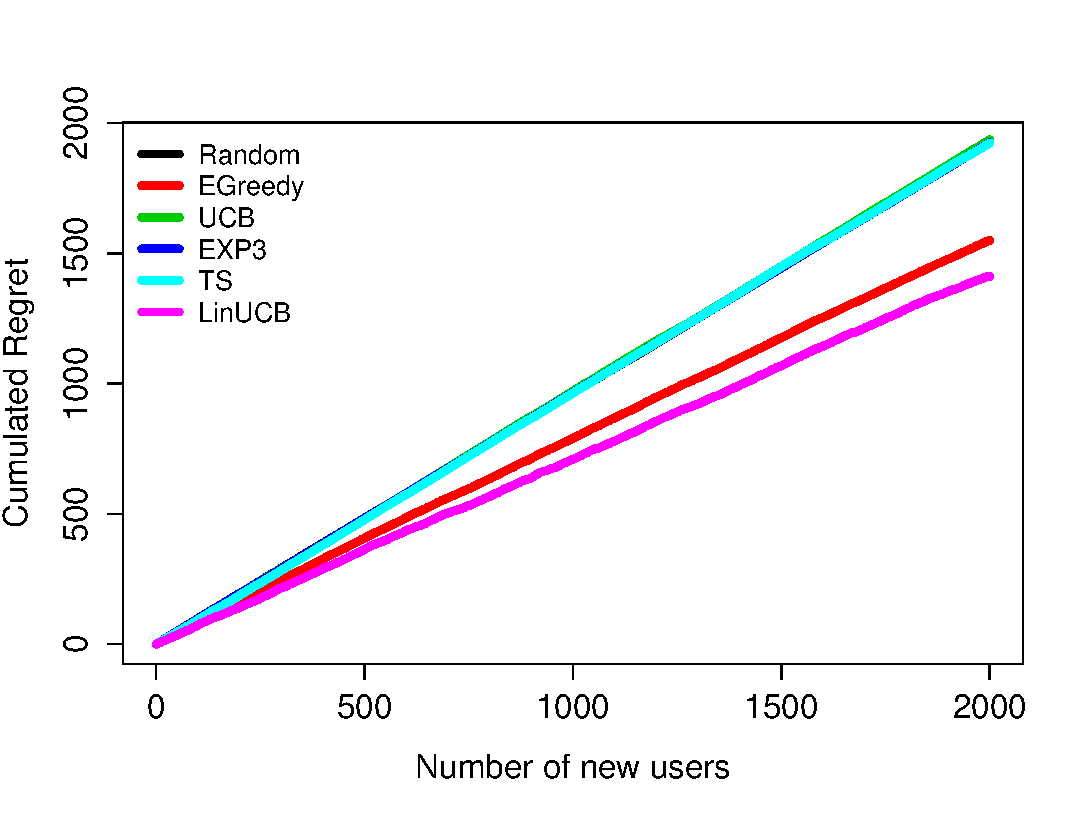
\includegraphics[width=.32\textwidth]{newSys-addedUser-Movielen.pdf}}
%\subfigure[New system on Netflix]{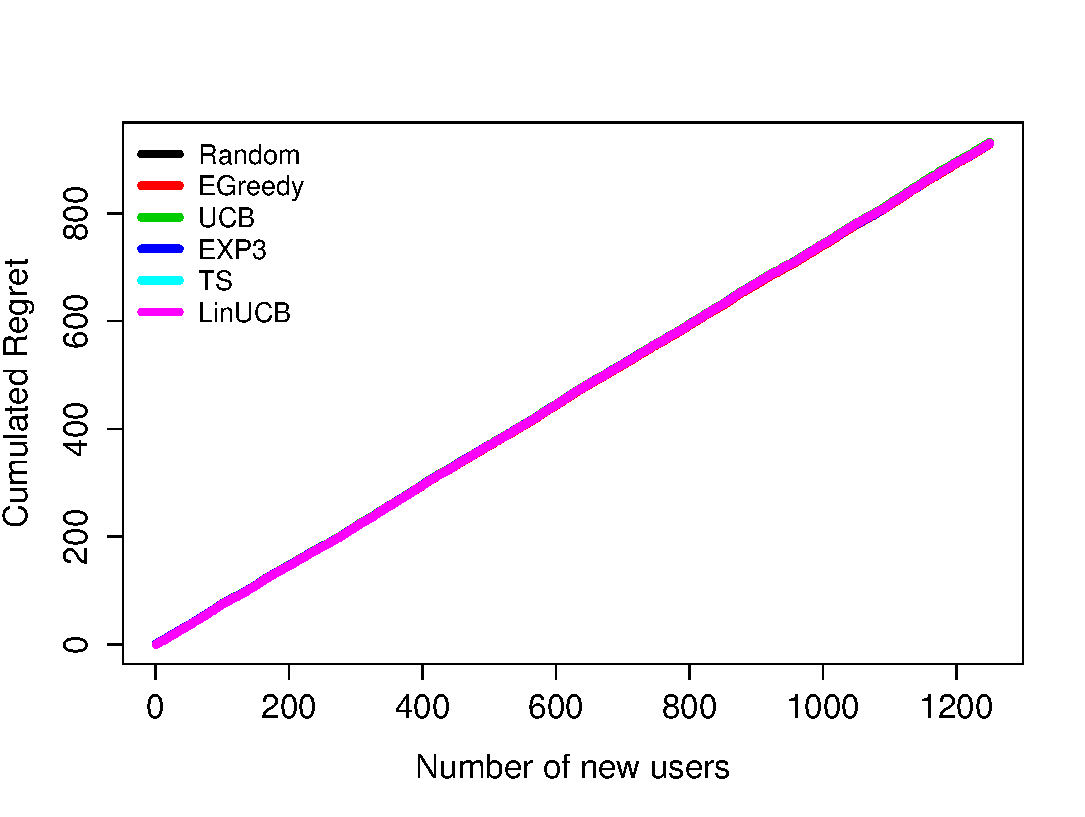
\includegraphics[width=.32\textwidth]{newSys-addedUser-Netflix.pdf}}
%\subfigure[New system on Yahoo!Music]{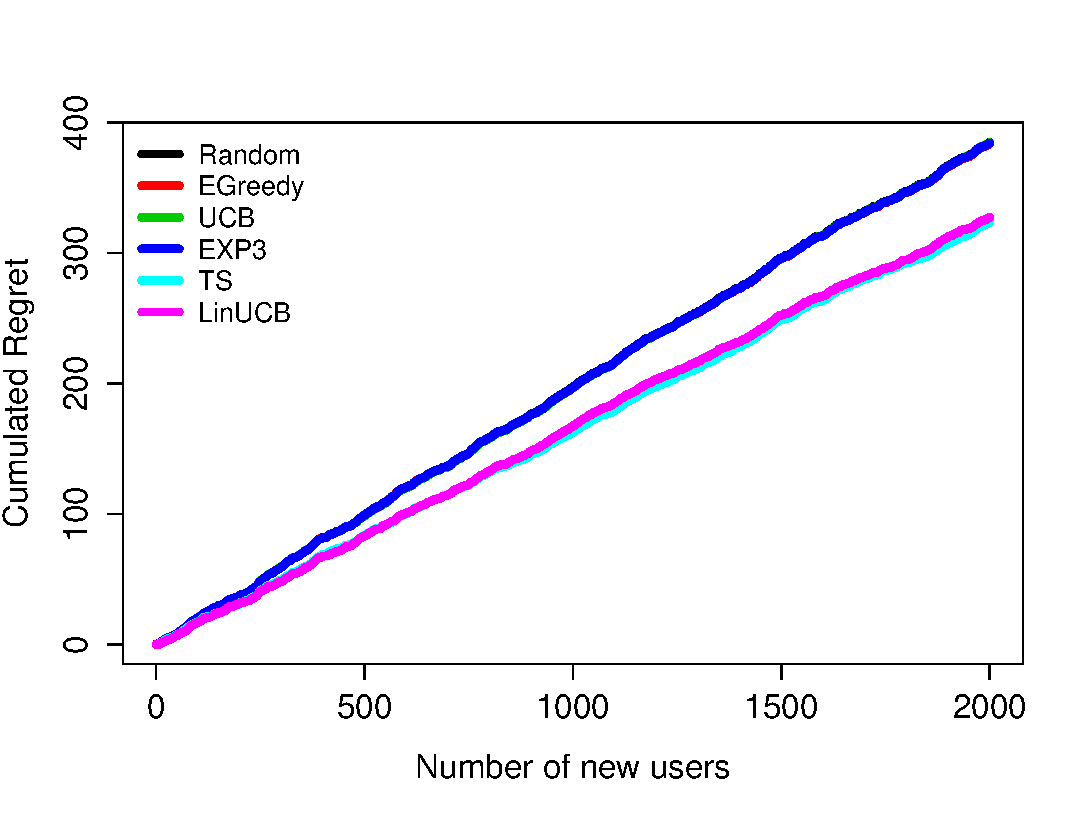
\includegraphics[width=.32\textwidth]{newSys-addedUser-Yahoo.pdf}}
%\end{center}
%\caption{Cumulative regrets for the complete new recommendation system, in which \textbf{we added new users}.}
%\label{fig:NewSysRecSys-addedUser}
%\end{figure*}
%%---------------------------------------------
%%Follow the new items
%\begin{table}
%\centering
%\begin{tabular}{|l|c|c|c|}
%\hline
%Methods & Movielen & Netflix & Yahoo!Music \\
%\hline
%Random & 1570.11 & 512.08 & 87.86 \\
%\hline
%EGreedy & 1474.08 & 512.2 & 88.11 \\
%\hline  
%UCB & 1569.79 & 513.2 & 87.76 \\
%\hline
%EXP3 & 1568.95 & 512.72 & 87.85 \\
%\hline
%TS & 1588.99 & 512.2 & 88.11 \\
%\hline
%LinUCB & 1268.6 & 512.2 & 88.11 \\
%\hline
%\end{tabular}
%\caption{Cumulative regrets for the complete new recommendation system, in which \textbf{we added new items}.}
%\end{table}
%%---------------------------------------------
%\begin{figure*}[ht!]
%\centering
%\begin{center}
%\subfigure[New system on Movielen]{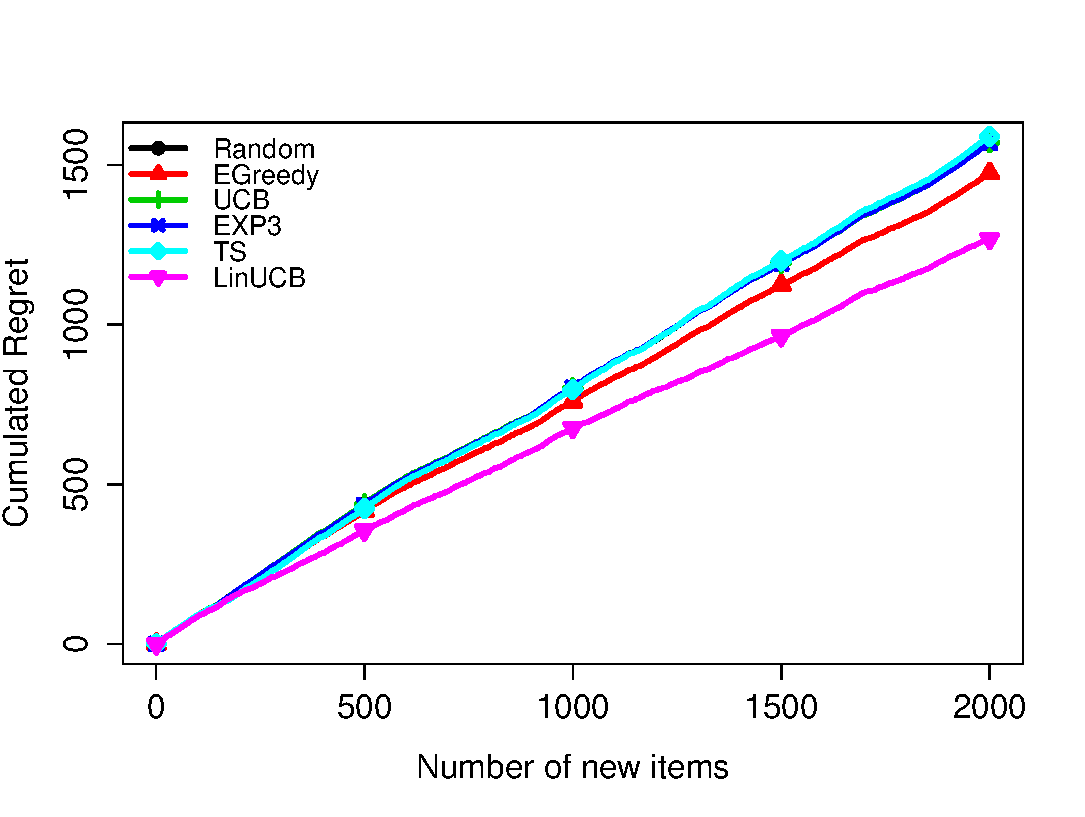
\includegraphics[width=.32\textwidth]{test.pdf}}%{newSys-addedItem-Movielen.pdf}}
%\subfigure[New system on Netflix]{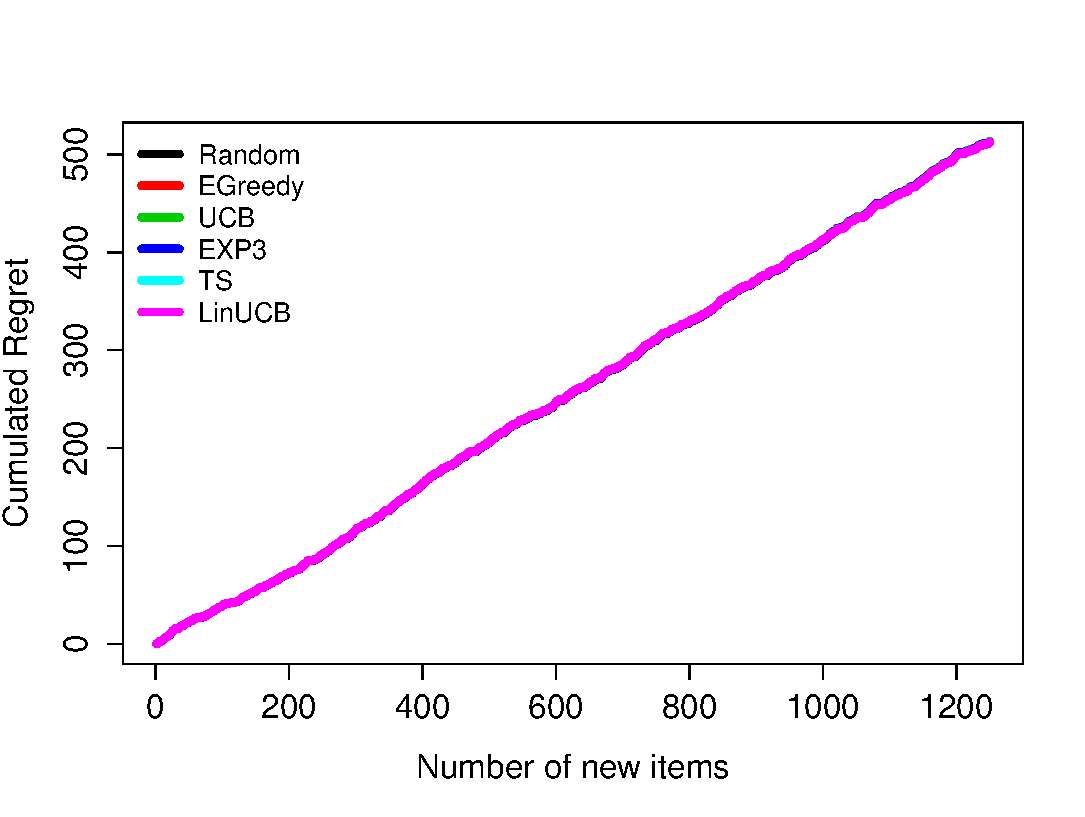
\includegraphics[width=.32\textwidth]{newSys-addedItem-Netflix.pdf}}
%\subfigure[New system on Yahoo!Music]{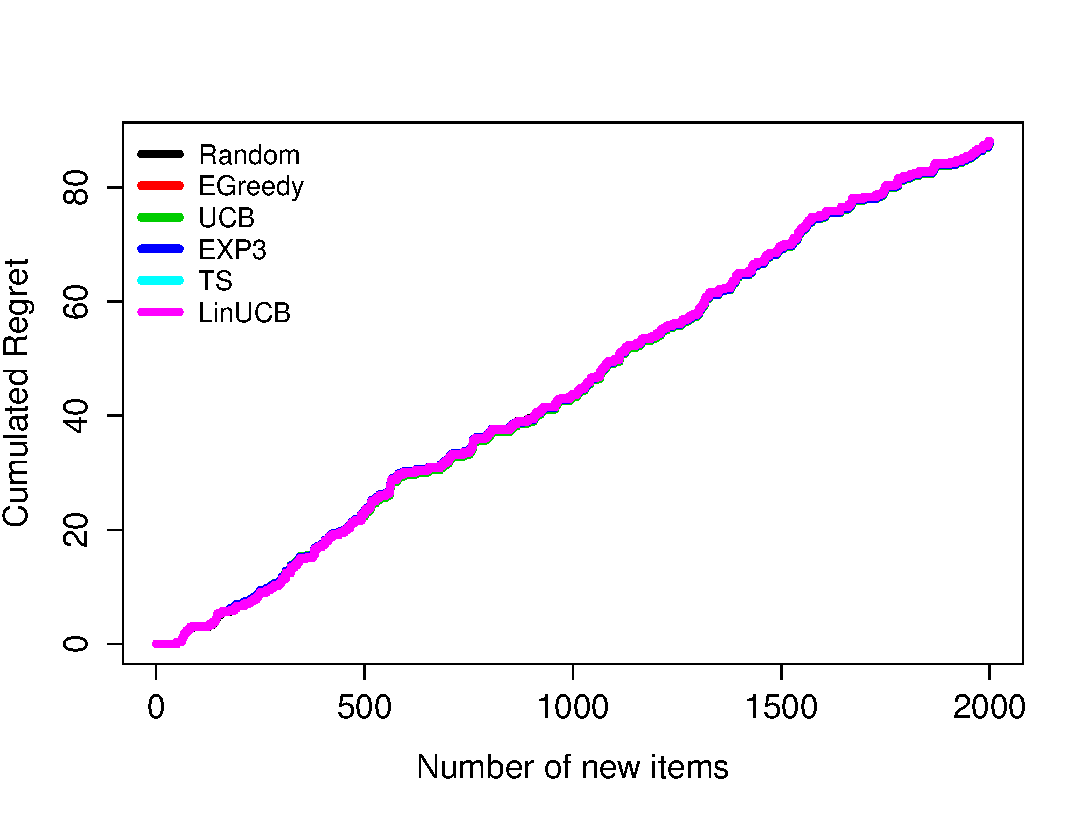
\includegraphics[width=.32\textwidth]{newSys-addedItem-Yahoo.pdf}}
%\end{center}
%\caption{Cumulative regrets for the complete new recommendation system, in which \textbf{we added new items}.}
%\label{fig:NewSysRecSys-addedItem}
%\end{figure*}

\subsubsection{Results on dealing with missing values}
~\\
We filled the missing values in the base matrix $X$ by using three approaches described above. We then ran the A-LinUCB algorithm with $\alpha=0.001$, which is the best choice in our experiments, on the matries $Y$ of the Movielen, Netflix and Yahoo!Music data sets. Finally, we measured the cumulative regrets of the new user recommendation systems. The Table~\ref{table:missingValuePerformance} shows the obtained performances.

It can be seen that the Average approach works best with smallest cumulative regret. The Zero method is slightly worse than the Average on the Movielen data set only, yet it gained more efficiency in terms of running time. Supprisingly, the impute SVD and the alternative SVD provided worst resutls in our experiments.

Over all, we decided to use the Zero approach for the further comparisons because of its performances and efficency.
%--------------Three methods to deal with missing values ---------------
%========================Performance=======================
\begin{table*}
  \caption{Cumulative regrets for the new user recommendation system to compare three different approaches in dealing with missing values, namely by zero value, by average value, by impute SVD and by alternative SVD.}
  \centering
  \begin{tabular}{|l|c|c|c|c|}
    \hline
    Dataset & By zero & By average & By impute SVD & By alt.SVD\\
    \hline
    Movielen & 3008.19 & 3006.8 & 4872 & 4869.2\\
    \hline
    Netflix & 3680 & 3680 & 3856 & 3856.8\\
    \hline  
    Yahoo!Music & 989.56 & 989.56 & 1143.81 & 1512.35\\
    \hline
  \end{tabular}
  \label{table:missingValuePerformance}
\end{table*}
%%========================Running time=======================
%\begin{table*}
%  \caption{Running time for the new user recommendation system to compare three different approaches in dealing with missing values, namely by zero value, by average value, by impute SVD and by alternative SVD.}
%  \centering
%  \begin{tabular}{|l|c|c|c|c|}
%    \hline
%    Dataset & By zero & By average & By impute SVD & By alt.SVD\\
%    \hline
%    Movielen & mins & mins & mins & mins\\
%    \hline
%    Netflix & mins & mins & mins & mins\\
%    \hline  
%    Yahoo!Music & mins & mins & mins & mins\\
%    \hline
%  \end{tabular}
%  \label{table:missingValueTime}
%\end{table*}

\subsubsection{Results on competing different methods}
~\\
As shown in Table~\ref{table:newUser} and Table~\ref{table:newItem}, obviously the random policy is much worse than the A-LinUCB in terms of the cumulative regrets. For example, in the cased of the new user recommendation system on the Yahoo!Music data set, the A-LinUCB algorithms provided a better performance than the random's result by 34\%.

%--------------For the new user problem ---------------
%For cumulative regret
\begin{table}
  \caption{Cumulative regrets for the \textbf{new user} recommendation system.}
  \centering
  \begin{tabular}{|l|c|c|c|}
    \hline
    Methods & Movielens & Netflix & Yahoo!Music \\
    \hline
    Random & 2024.26 & 3852 & 1514.30\\
    \hline
    Aver & 1255 & 3825 & 1125.15 \\
    \hline
    EGreedy & 1218.4 & 3758.66 & 1108.97 \\
    \hline  
    UCB & 1973.3 & 3850.86 & 1514.77 \\
    \hline
    EXP3 & 1868.4 & 3836.66 & 1276.42 \\
    \hline
    %TS & 3822 & 3854 & 1313.70 \\
    %\hline
     LinUCB & 1595.86 & 3732.86 & 1325.86 \\
    \hline
    A-LinUCB & 1069.8 & 3659.4 & 989.92 \\
    \hline
  \end{tabular}
  \label{table:newUser}
\end{table}

%For running time
\begin{table}
  \caption{Running time of the \textbf{new user} recommendation system (in seconds).}
  \centering
  \begin{tabular}{|l|c|c|c|}
    \hline
    Methods & Movielens & Netflix & Yahoo!Music \\
    \hline
    Random & 93 &  15.16& 12.43\\
    \hline
    Aver & 117 & 21.9 & 18.44 \\
    \hline
    EGreedy & 113 & 22.12 & 18.57\\
    \hline  
    UCB & 48.96 & 22.39 & 18.77\\
    \hline
    EXP3 & 38.28 & 23.43 & 19.12\\
    \hline
    %TS &  &  & \\
    %\hline
     LinUCB & 20214 & 2361.6 & 2448 \\
    \hline
    A-LinUCB & 5184 & 654 & 612\\
    \hline
  \end{tabular}
  \label{table:newUserTime}
\end{table}


%---------------------------------------------
\begin{figure*}[ht!]
  \centering
  \begin{center}
    \subfigure[Movielens with size $6040\times 3952$. ]{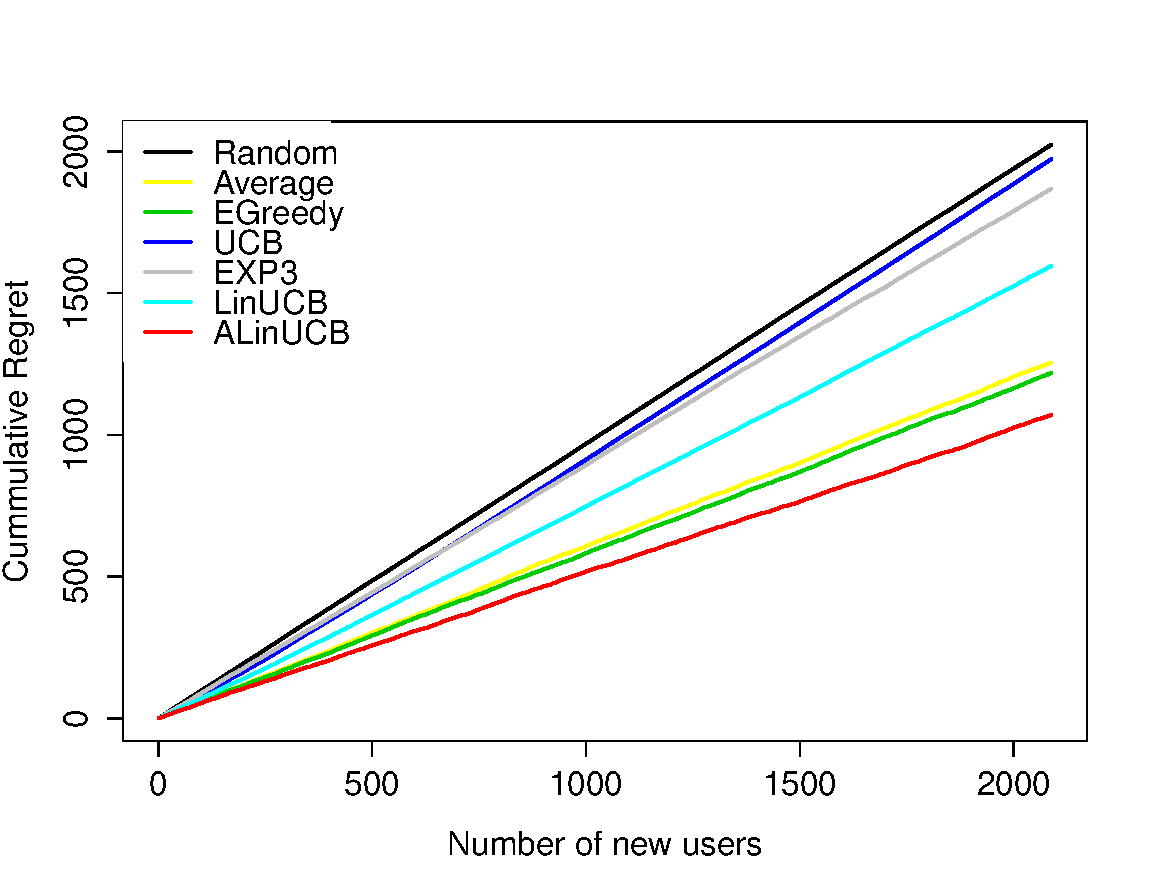
\includegraphics[width=.3\textwidth]{newUser-Movielen.pdf}}
    \subfigure[Netflix with size $6423\times 1250$ ]{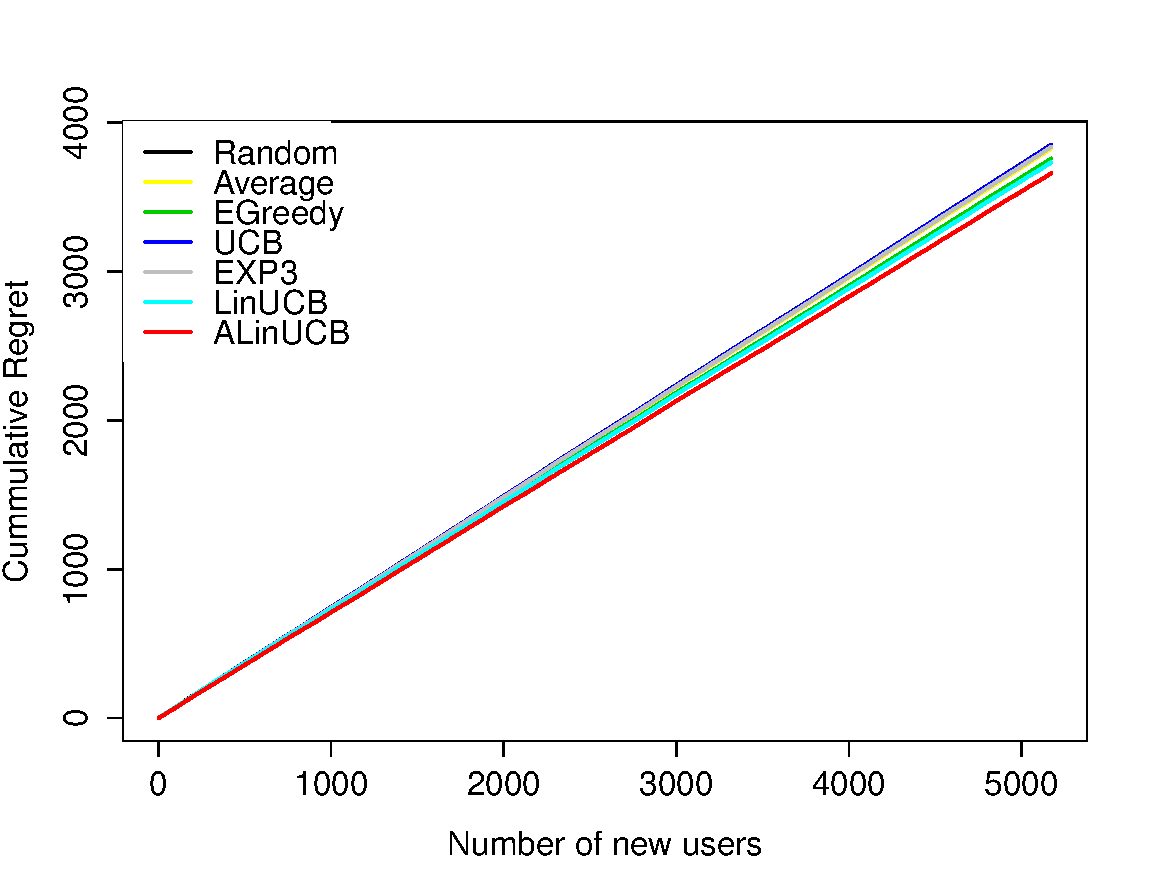
\includegraphics[width=.3\textwidth]{newUser-Netflix.pdf}}
    \subfigure[Yahoo!Music with size $10,000\times 1000$]{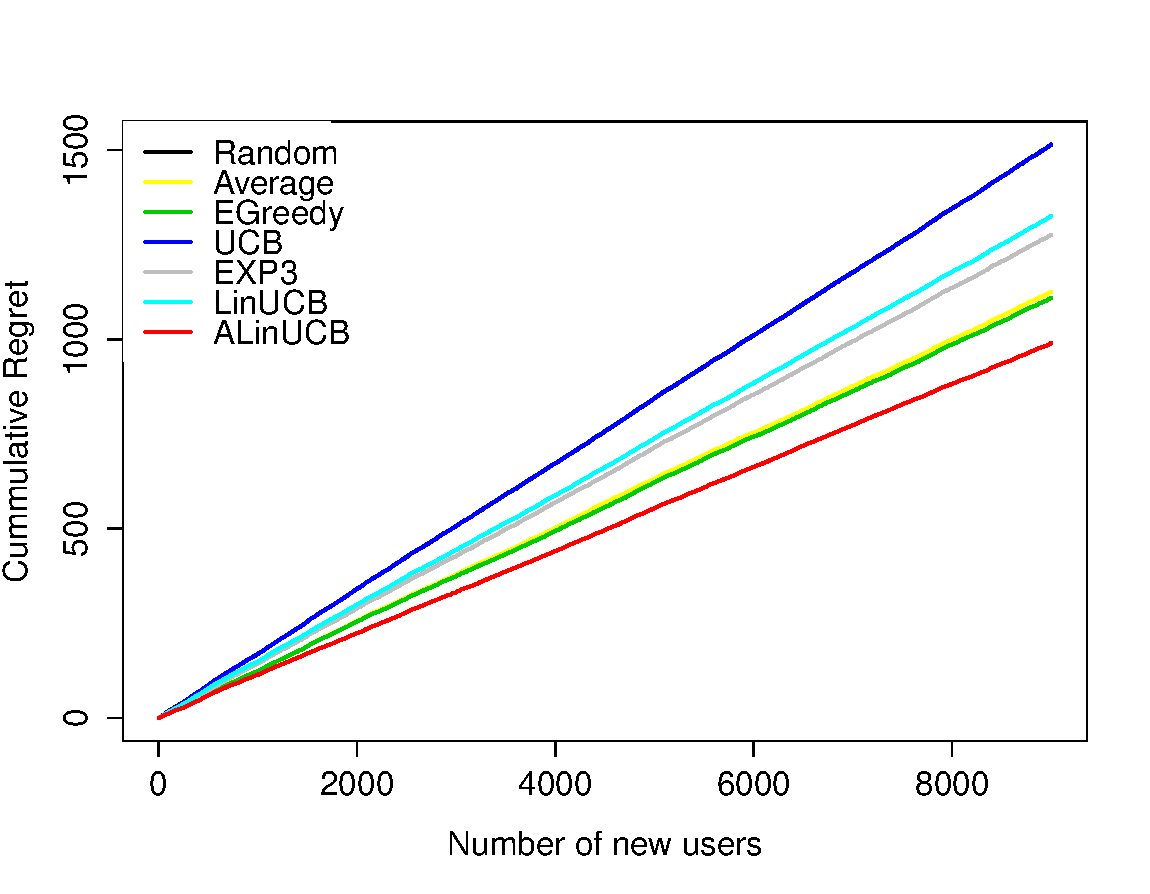
\includegraphics[width=.3\textwidth]{newUser-Yahoo.pdf}}
  \end{center}
  \caption{Cumulative regrets for the \textbf{new user} recommendation systems. Several curses are hidden on the graphs as the performances of these methods is almost the same.}
  \label{fig:newUser}
\end{figure*}

%----------------For the new item problem-----------
%For cumulative regret
\begin{table}
  \caption{Cumulative regrets for the \textbf{new item} recommendation system.}
  \centering
  \begin{tabular}{|l|c|c|c|}
    \hline
    Methods & Movielens & Netflix & Yahoo!Music \\
    \hline
    Random & 2226.5 & 179.6 & 314.59\\
    \hline
    Aver & 1721.86 & 179.6 & 285 \\
    \hline
    EGreedy & 1664.46 & 178.06 & 273.81 \\
    \hline  
    UCB & 2221.46 & 179.93 & 313.75 \\
    \hline
    EXP3 & 2133.19 & 179.2 & 306.92 \\
    \hline
    %TS & 2170.79 & 168.8 & 318.96 \\
    %\hline
     LinUCB & 1715.73 & 173.46 & 273.24 \\
    \hline
    A-LinUCB & 1645.46 & 169.6 & 266.95 \\
    \hline
  \end{tabular}
  \label{table:newItem}
\end{table}

%For running time
\begin{table}
  \caption{Running time of the \textbf{new item} recommendation system (in seconds).}
  \centering
  \begin{tabular}{|l|c|c|c|}
    \hline
    Methods & Movielens & Netflix & Yahoo!Music \\
    \hline
    Random & 35.36 & 0.94 & 12.26\\
    \hline
    Aver & 47.75 & 1.49 & 18.28 \\
    \hline	
    EGreedy & 45.29 & 1.46 & 18.41\\
    \hline  
    UCB & 35.62 & 1.43 & 18.67\\
    \hline
    EXP3 & 30.32 & 1.46 & 19.59\\
    \hline
    %TS &  &  & \\
    %\hline
     LinUCB & 2325.27 & 57.5 & 2866.68 \\
    \hline
    A-LinUCB & 547.75 & 13.8 & 360\\
    \hline
  \end{tabular}
  \label{table:newItemTime}
\end{table}
%---------------------------------------------
\begin{figure*}[ht!]
  \centering
  \begin{center}
    \subfigure[Movielens with size $1000\times 3952$]{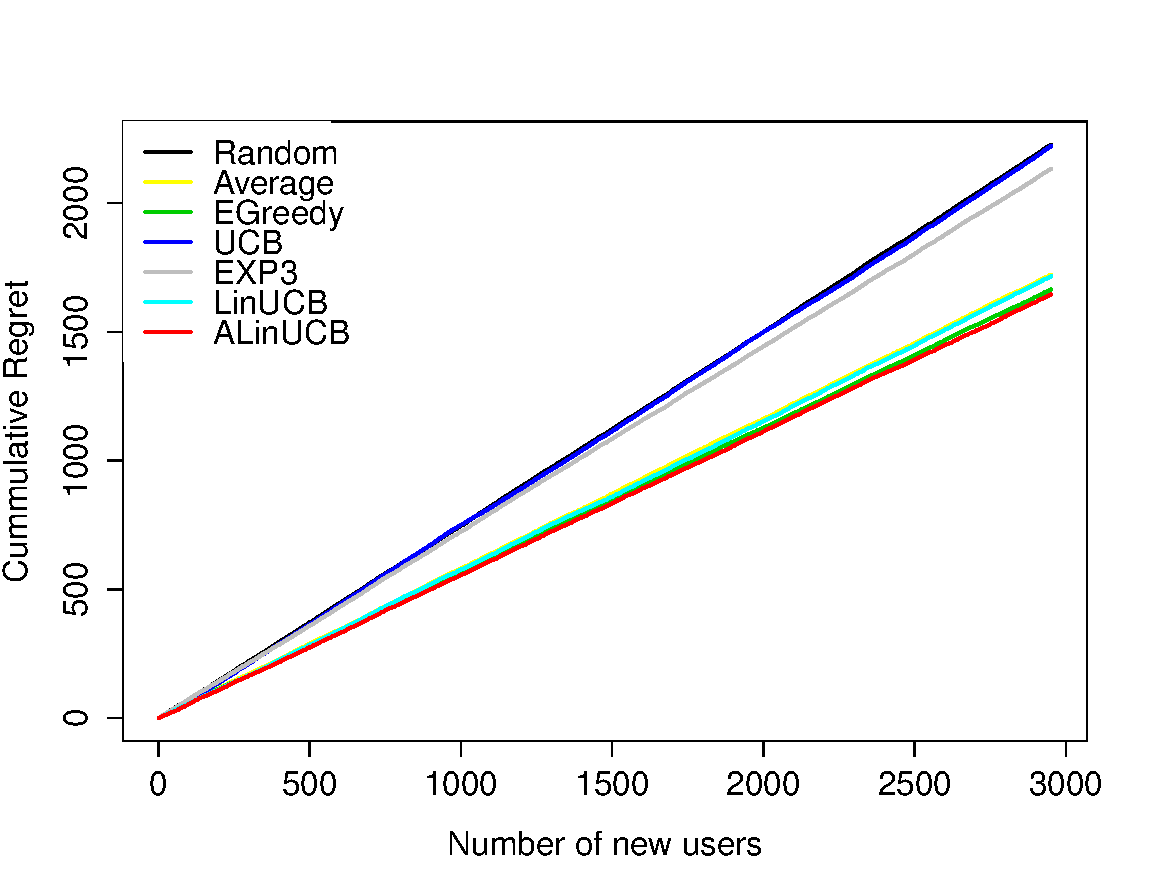
\includegraphics[width=.3\textwidth]{newItem-Movielen.pdf}}
    \subfigure[Netflix with size $500\times 1250$]{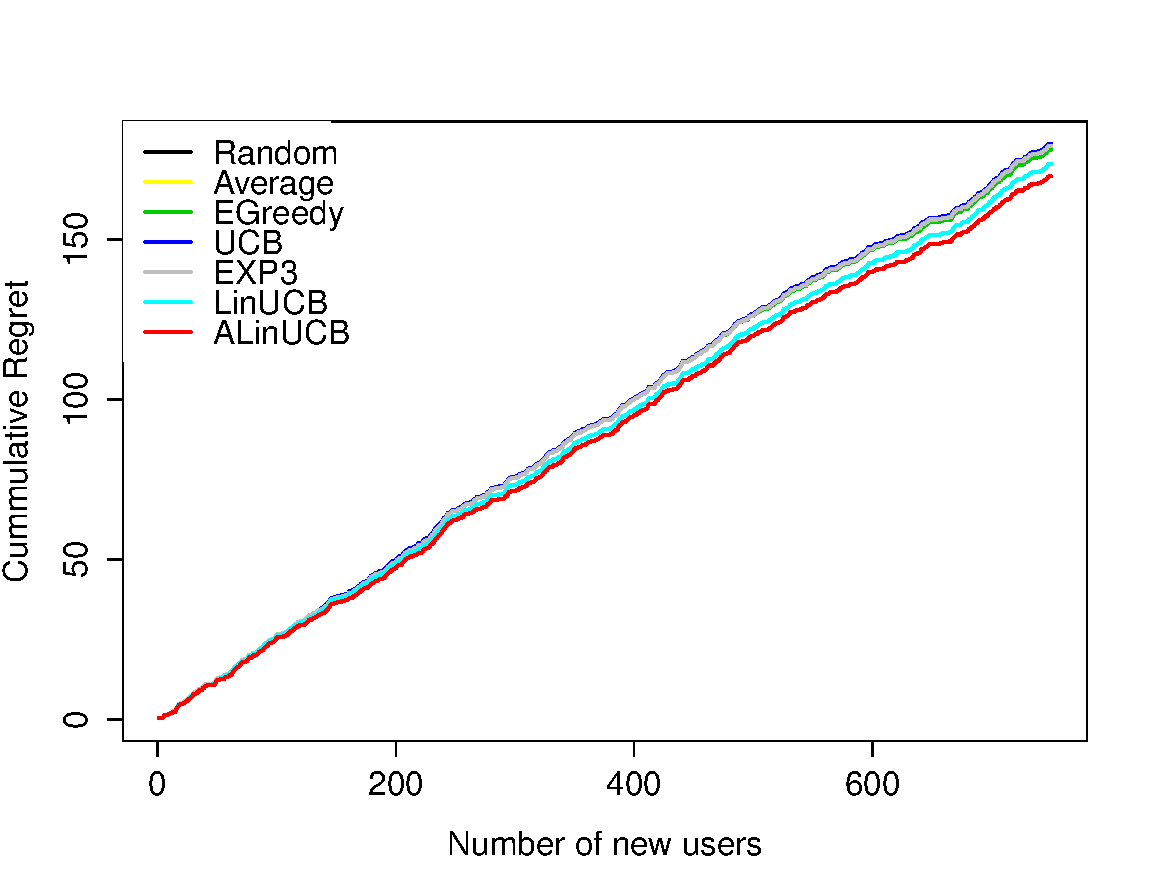
\includegraphics[width=.3\textwidth]{newItem-Netflix.pdf}}
    \subfigure[Yahoo!Music with size $1000\times 10,000$]{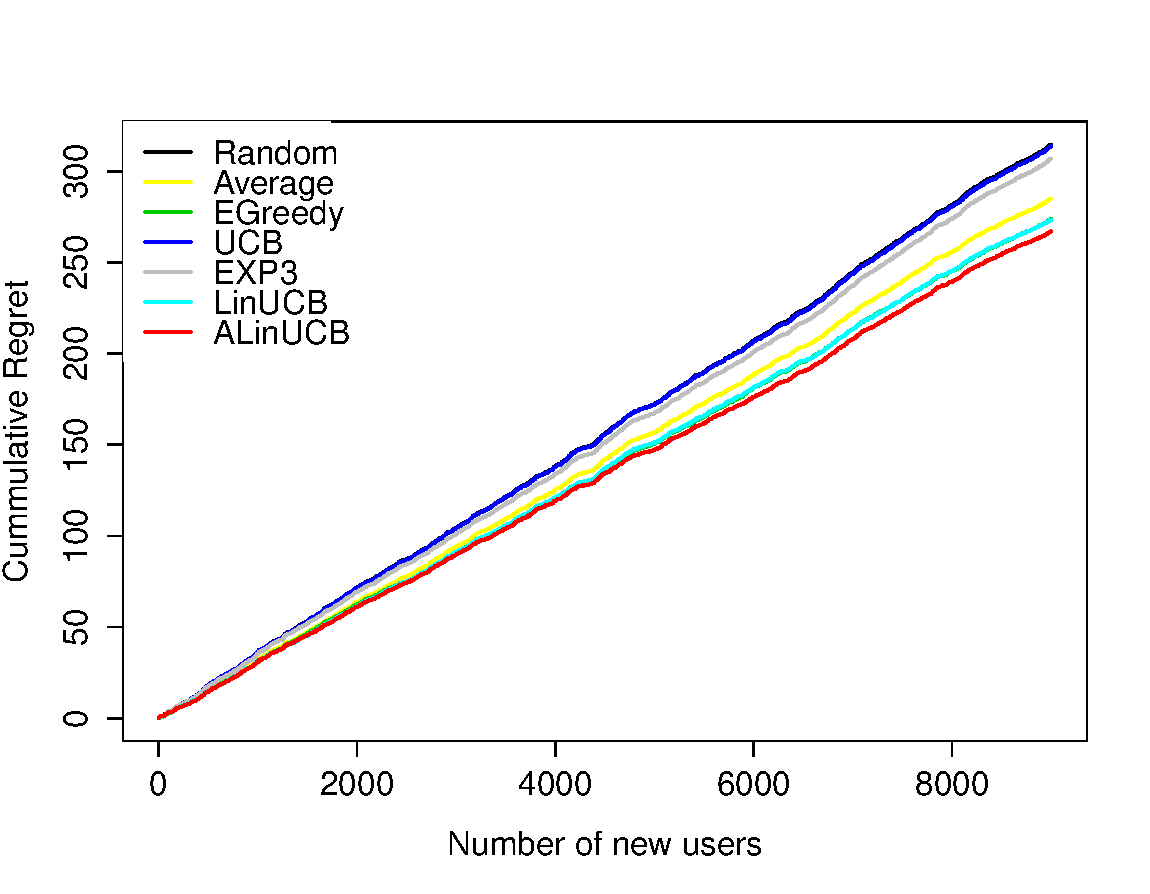
\includegraphics[width=.3\textwidth]{newItem-Yahoo.pdf}}
  \end{center}
  \caption{Cumulative regrets for the \textbf{new item} recommendation systems. Several curses are hidden on the graphs as the performances of these methods is almost the same.}
  \label{fig:newItem}
\end{figure*}
Clearly, with no use of the information about previous ratings the UCB and EXP3 algorithms
performed almost the same like the random strategy. Even the EXP3 is the worst choice in terms of
the cumulative regret and the running time. The EG algorithm is exceptional since its performance
is much better than the UCB and EXP3, yet still lower than the A-LinUCB. This can be explained by
the fact that an item, which is preferred by an enough number of users, will likely be a good
choice for the others. The greedy EG strategy has fully utilized this character of a recommendation
systems to provide good results. For instance, in the case of the new movie recommendation system
built on the Movielens data set, the EG policy performed very well with almost 10\% better than the
random strategy.

With the Thompson sampling (TS) policy, we got better results than the Random, UCB and EXP3. This illustrated that the information of previous ratings contributed to the better recommendation results. However, its performance is still lower than the EG and A-LinUCB. Therefore, we can conclude that the context information must be used in an appropriate way, which is the A-LinUCB as a sample in our experiments. 

It can be seen from the Table~\ref{table:A-LinUCB(0)vsA-LinUCB(0.001)} that the A-LinUCB algorithm with $\alpha=0$ performed much worse than the A-LinUCB when $\alpha=0.001$ on all three data sets. That means a little exploration helped to provide better results in solving cold-start recommendation systems. 

%---------Cummulative regret: A-LinUCB(alpha=0) vs A-LinUCB(alpha=0.001)
\begin{table}
  \caption{Cumulative regrets for new user recommendation system to
    compare between A-LinUCB ($\alpha=0$) with A-LinUCB
    ($\alpha=0.001$).}
  \centering
  \begin{tabular}{|l|c|c|c|}
    \hline
    A-LinUCB & Movielens & Netflix & Yahoo!Music \\
    \hline
    $\alpha=0$ & 3491.39 & 3857 & 1514.15 \\
    \hline
    $\alpha=0.001$ & 3008.19 & 3680 & 989.56 \\
    \hline
  \end{tabular}
  \label{table:A-LinUCB(0)vsA-LinUCB(0.001)}
\end{table}


%%-----------Cumulative regret: A-LinUCB vs. Stand.LinUCB
%\begin{table}
%  \caption{Cumulative regrets for new user recommendation system to compare between the standard LinUCB and the A-LinUCB.}
%  \centering
%  \begin{tabular}{|l|c|c|c|}
%    \hline
%    Methods & Movielen & Netflix & Yahoo!Music \\
%    \hline
%    Stand.LinUCB & 4717.4 & 3855.2 & 1478.6 \\
%    \hline
%    A-LinUCB & 3008.19 & 3680 & 989.56 \\
%    \hline
%  \end{tabular}
%  \label{table:A-LinUCBvsStand-LinUCB-Performance}
%\end{table}
%
%%------------Time running: A-LinUCB vs. Stand.LinUCB
%\begin{table}
%  \caption{Running time to compare between the standard LinUCB and the A-LinUCB.}
%  \centering
%  \begin{tabular}{|l|c|c|c|}
%    \hline
%    Methods & Movielen & Netflix & Yahoo!Music \\
%    \hline
%    Stand.LinUCB & 49 mins & 41 mins & 49 mins \\
%    \hline
%    A-LinUCB & 4.5 mins & 4 mins & 5 mins \\
%    \hline
%  \end{tabular}
%  \label{table:A-LinUCBvsStand-LinUCB-Time}	  
%\end{table}

%-----------Related work--------
\section{Related work}

The cold-start problem was readily identified as of the emergence of recommendation
systems~\cite{Schein:2002:MMC:564376.564421}. Along time, several solutions for these problems were
proposed. However, these approaches depend strongly on side information available on the users and
items, which is not always available. Therefore, it is very hard to build accurate recommendation
systems in practice, despite the strong activity on the subject. For example, the
work~\cite{Lashkari94collaborativeinterface} suggested an interview process with users to gather
more information about their preferences before the actual recommendations. Recently, a lot of
works have been conducted to improve the estimation speed of the parameters for new items or new
users by using hierarchy of items or various side
informations~\cite{DBLP:conf/nips/AgarwalCEMPRRZ08,contextualRecommendation,Agarwal:2009:SME:1526709.1526713}. The augmentation with information mined from social networks is also a common approach
today.

Another common strategy to mitigate the cold-start user problem is to gather demographic data. It is assume that users who share a common background also share a common taste in products. Examples include Lekakos and Giaglis \cite{lekakos07}, where lifestyle information is employed. This includes age, marital status and education, as well as preferences on eight television genres. Correlation between users are found by applying the Pearson correlation coefficient. The authors report that this approach is the most effective way of dealing with the cold-start user problem in sparse environments.

A similar thought underlies the work by Lam et al., \cite{lam08:_addres} where an \textit{aspect model} (see e.g. \cite{marlin04:_collab}) including age, gender and job is used. This information is used to calculate a probability model that classifies users into user groups and the probability how well liked an item is by this user group. 

Other examples of applying demographic information to mitigate the cold-start user problem exists, e.g. \cite{gao07:_person,agarwal09:_regres,park09:_pairw}. All the the solution above use similar demographic information; most commonly age, occupation and gender. Most of the solutions asked for less that five pieces of information. Even though five is a comparatively small number, the user must still answer these questions. Users do generally not like to answer a lot of questions, yet expect reasonable performance from the first interaction with the user \cite{zigoris06:_bayes}. 

Zigoris and Zhang \cite{zigoris06:_bayes}, suggests to use a two part Bayesian model, where the prior probability is based on the existing user population and \textit{data likelihood}, which is based on the data supplied by the user. Thus, when a new user enters the system, little is know about that user and the prior distribution is the main contributor. As the user interacts with the system the data data likelihood becomes more and more important. This approach performs well for cold-start users. Other similar approaches can by found in \cite{manavoglu03:_probab}, suggesting a Markov mixture model and \cite{xue09:_user}, who suggests a statical user language model that integrates an individual model, a group model and a global model.

In this paper, we consider this problem from a different
perspective. Though perfectly aware of the potential utility of side
information, we consider the problem without any side information,
only focussing on acquiring appetence of new users and appeal new
items as fast as possible with as few as possible ``bad'' recommendations.
%\hai{Can you add some thing more here...?}.\jm{done} 
%As shown in above sections, our proposed framework makes no use of any additional information on the users and items. It utilizes only the previous ratings as the context information, which is always possible and easily captured in real recommendation systems.

%------------------- Conclusions and future study ---------------------- 
\section{Conclusions and future study} 

The main focus of this paper is on cold-start problems in recommendation systems. We
have casted these problems as contextual-bandit problems and adapted LinUCB to solve
them. We have conducted performance analysis of the proposed A-LinUCB algorithms and compared it
with six different approaches: random policy, $\epsilon$-greedy, UCB, EXP3, Thompson sampling and
A-LinUCB($\alpha=0$). We have used three data sets from Movielens, Netflix and Yahoo!Music and the
performance of algorithms were measured by the cumulative regret. Our proposed A-LinUCB algorithms
have clearly demonstrated better results than all the others in both new user and new item
recommendation systems. As proposed in this paper, A-LinUCB requires no side information on users and items; A-LinUCB may be extended to take advantage of such sources of information; this is left as future work. %Moreover, we demonstrate the efficiency in handling a large numbers of users/items.

There are two main directions for future works: first, it would be interesting to extend the proposed framework to solve the cold-start system problem, where we have completely new users and new items. Second, we plan to study another forms of the cumulative regret for the case when only implicit feedbacks of users are available, such as clicks or browsing. 
%------------------- ACK ----------------------
%\section{Acknowledgments}
%This work was supported by Ministry of Higher Education and Research,
%Nord-Pas-de-Calais Regional Council and FEDER through the' Contrat de Projets Etat Region (CPER) 2007-2013' and Carnot program of Inria.
%\jm{LAMPADA ??? Other ? }
%------------------- Reference ----------------------
\bibliographystyle{plain}
\bibliography{ref}

\end{document}


%------------------------------ For edition -------------------------------------

%\section{Problem Specification.}In this paper, we consider the solution of the $N \times
%N$ linear
%system
%\begin{equation} \label{e1.1}
%A x = b
%\end{equation}
%where $A$ is large, sparse, symmetric, and positive definite.  We consider
%the direct solution of (\ref{e1.1}) by means of general sparse Gaussian
%elimination.  In such a procedure, we find a permutation matrix $P$, and
%compute the decomposition
%\[
%P A P^{t} = L D L^{t}
%\]
%where $L$ is unit lower triangular and $D$ is diagonal.  
%
% 
%\section{Design Considerations.}Several good ordering algorithms (nested dissection and
%minimum degree)
%are available for computing $P$  \cite{GEORGELIU}, \cite{ROSE72}.
%Since our interest here does not
%focus directly on the ordering, we assume for convenience that $P=I$,
%or that $A$ has been preordered to reflect an appropriate choice of $P$.
%
%Our purpose here is to examine the nonnumerical complexity of the
%sparse elimination algorithm given in  \cite{BANKSMITH}.
%As was shown there, a general sparse elimination scheme based on the
%bordering algorithm requires less storage for pointers and
%row/column indices than more traditional implementations of general
%sparse elimination.  This is accomplished by exploiting the m-tree,
%a particular spanning tree for the graph of the filled-in matrix.
%
%\begin{theorem} The method  was extended to three
%dimensions. For the standard multigrid
%coarsening
%(in which, for a given grid, the next coarser grid has $1/8$
%as many points), anisotropic problems require plane
%relaxation to
%obtain a good smoothing factor.\end{theorem} 
%
%Our purpose here is to examine the nonnumerical complexity of the
%sparse elimination algorithm given in  \cite{BANKSMITH}.
%As was shown there, a general sparse elimination scheme based on the
%bordering algorithm requires less storage for pointers and
%row/column indices than more traditional implementations of general
%sparse elimination.  This is accomplished by exploiting the m-tree,
%a particular spanning tree for the graph of the filled-in matrix.
%Several good ordering algorithms (nested dissection and minimum degree)
%are available for computing $P$  \cite{GEORGELIU}, \cite{ROSE72}.
%Since our interest here does not
%focus directly on the ordering, we assume for convenience that $P=I$,
%or that $A$ has been preordered to reflect an appropriate choice of $P$.
%
%\begin{proof} In this paper we consider two methods. The first method
%is
%basically the method considered with two differences:
%first, we perform plane relaxation by a two-dimensional
%multigrid method, and second, we use a slightly different
%choice of
%interpolation operator, which improves performance
%for nearly singular problems. In the second method coarsening
%is done by successively coarsening in each of the three
%independent variables and then ignoring the intermediate
%grids; this artifice simplifies coding considerably.
%\end{proof}
%
%Our purpose here is to examine the nonnumerical complexity of the
%sparse elimination algorithm given in  \cite{BANKSMITH}.
%As was shown there, a general sparse elimination scheme based on the
%bordering algorithm requires less storage for pointers and
%row/column indices than more traditional implementations of general
%sparse elimination.  This is accomplished by exploiting the m-tree,
%a particular spanning tree for the graph of the filled-in matrix.
%
%\begin{Definition}{\rm We describe the two methods in \S 1.2. In \S\ 1.3. we
%discuss
%some remaining details.}
%\end{Definition}
%
%Our purpose here is to examine the nonnumerical complexity of the
%sparse elimination algorithm given in  \cite{BANKSMITH}.
%As was shown there, a general sparse elimination scheme based on the
%bordering algorithm requires less storage for pointers and
%row/column indices than more traditional implementations of general
%sparse elimination.  This is accomplished by exploiting the m-tree,
%a particular spanning tree for the graph of the filled-in matrix.
%Several good ordering algorithms (nested dissection and minimum degree)
%are available for computing $P$  \cite{GEORGELIU}, \cite{ROSE72}.
%Since our interest here does not
%focus directly on the ordering, we assume for convenience that $P=I$,
%or that $A$ has been preordered to reflect an appropriate choice of $P$.
%
%Our purpose here is to examine the nonnumerical complexity of the
%sparse elimination algorithm given in  \cite{BANKSMITH}.
%As was shown there, a general sparse elimination scheme based on the
%bordering algorithm requires less storage for pointers and
%row/column indices than more traditional implementations of general
%sparse elimination.  
%
%\begin{lemma} We discuss first the choice for $I_{k-1}^k$
%which is a generalization. We assume that $G^{k-1}$ is
%obtained
%from $G^k$
%by standard coarsening; that is, if $G^k$ is a tensor product
%grid $G_{x}^k \times G_{y}^k \times G_{z}^k$,
%$G^{k-1}=G_{x}^{k-1} \times G_{y}^{k-1} \times G_{z}^{k-1}$,
%where $G_{x}^{k-1}$ is obtained by deleting every other grid
%point of $G_x^k$ and similarly for $G_{y}^k$ and $G_{z}^k$.
%\end{lemma}
% 
%To our knowledge, the m-tree previously has not been applied in this
%fashion to the numerical factorization, but it has been used,
%directly or indirectly, in several optimal order algorithms for
%computing the fill-in during the symbolic factorization phase
%[4] - [10], [5], [6]. In \S 1.3., we analyze the complexity of the old and new
%approaches to the intersection problem for the special case of
%an $n \times n$ grid ordered by nested dissection. The special
%structure of this problem allows us to make exact estimates of
%the complexity. To our knowledge, the m-tree previously has not been applied in this
%fashion to the numerical factorization, but it has been used,
%directly or indirectly, in several optimal order algorithms for
%computing the fill-in during the symbolic factorization phase
%[4] - [10], [5], [6].
%
%In \S 1.2, we review the bordering algorithm, and introduce
%the sorting and intersection problems that arise in the
%sparse formulation of the algorithm.  
%In \S 1.3., we analyze the complexity of the old and new
%approaches to the intersection problem for the special case of
%an $n \times n$ grid ordered by nested dissection. The special
%structure of this problem allows us to make exact estimates of
%the complexity. To our knowledge, the m-tree previously has not been applied in this
%fashion to the numerical factorization, but it has been used,
%directly or indirectly, in several optimal order algorithms for
%computing the fill-in during the symbolic factorization phase
%[4] - [10], [5], [6].
%
%
%For the old approach, we show that the
%complexity of the intersection problem is $O(n^{3})$, the same
%as the complexity of the numerical computations.  For the
%new approach, the complexity of the second part is reduced to
%$O(n^{2} (\log n)^{2})$.  
%
%To our knowledge, the m-tree previously has not been applied in this
%fashion to the numerical factorization, but it has been used,
%directly or indirectly, in several optimal order algorithms for
%computing the fill-in during the symbolic factorization phase
%[4] - [10], [5], [6]. In \S 1.3., we analyze the complexity of the old and new
%approaches to the intersection problem for the special case of
%an $n \times n$ grid ordered by nested dissection. The special
%structure of this problem allows us to make exact estimates of
%the complexity. To our knowledge, the m-tree previously has not been applied in this
%fashion to the numerical factorization, but it has been used,
%directly or indirectly, in several optimal order algorithms for
%computing the fill-in during the symbolic factorization phase
%[4] - [10], [5], [6].
%This is accomplished by exploiting the m-tree,
%a particular spanning tree for the graph of the filled-in matrix.
%To our knowledge, the m-tree previously has not been applied in this
%fashion to the numerical factorization, but it has been used,
%directly or indirectly, in several optimal order algorithms for
%computing the fill-in during the symbolic factorization phase
%\cite{EISENSTAT} - \cite{LIU2}, \cite{ROSE76},  \cite{SCHREIBER}.
%
%\subsection{Robustness.}We do not
%attempt to present an overview
%here, but rather attempt to focus on those results that
%are relevant to our particular algorithm.
%This section assumes prior knowledge of the role of graph theory
%in sparse Gaussian elimination; surveys of this role are
%available in \cite{ROSE72} and \cite{GEORGELIU}. More general
%discussions of elimination trees are given in
%\cite{LAW} - \cite{LIU2}, \cite{SCHREIBER}.
%Thus, at the $k$th stage, the bordering algorithm consists of
%solving the lower triangular system
%\begin{equation} \label{1.2}
% L_{k-1}v = c
%\end{equation}
%and setting
%\begin{eqnarray} 
%\ell &=& D^{-1}_{k-1}v , \\
%\delta &=& \alpha - \ell^{t} v .
%\end{eqnarray}
%
%\begin{figure}
%\vspace{14pc}
%\caption{This is a figure 1.1.}
%\end{figure}
%
%\section{Robustness.} We do not
%attempt to present an overview
%here, but rather attempt to focus on those results that
%are relevant to our particular algorithm.
% 
%\subsection{Versatility.}The special
%structure of this problem allows us to make exact estimates of
%the complexity.  For the old approach, we show that the
%complexity of the intersection problem is $O(n^{3})$, the same
%as the complexity of the numerical computations
%\cite{GEORGELIU}, \cite{ROSEWHITTEN}.  For the
%new approach, the complexity of the second part is reduced to
%$O(n^{2} (\log n)^{2})$. 
%
%To our knowledge, the m-tree previously has not been applied in this
%fashion to the numerical factorization, but it has been used,
%directly or indirectly, in several optimal order algorithms for
%computing the fill-in during the symbolic factorization phase
%[4] - [10], [5], [6]. In \S 1.3., we analyze the complexity of the old and new
%approaches to the intersection problem for the special case of
%an $n \times n$ grid ordered by nested dissection. The special
%structure of this problem allows us to make exact estimates of
%the complexity. To our knowledge, the m-tree previously has not been applied in this
%fashion to the numerical factorization, but it has been used,
%directly or indirectly, in several optimal order algorithms for
%computing the fill-in during the symbolic factorization phase
%[4] - [10], [5], [6].
%
%In \S 1.2, we review the bordering algorithm, and introduce
%the sorting and intersection problems that arise in the
%sparse formulation of the algorithm.  
%In \S 1.3., we analyze the complexity of the old and new
%approaches to the intersection problem for the special case of
%an $n \times n$ grid ordered by nested dissection. The special
%structure of this problem allows us to make exact estimates of
%the complexity. To our knowledge, the m-tree previously has not been applied in this
%fashion to the numerical factorization, but it has been used,
%directly or indirectly, in several optimal order algorithms for
%computing the fill-in during the symbolic factorization phase
%[4] - [10], [5], [6].
%
%
%For the old approach, we show that the
%complexity of the intersection problem is $O(n^{3})$, the same
%as the complexity of the numerical computations.  For the
%new approach, the complexity of the second part is reduced to
%$O(n^{2} (\log n)^{2})$.  
%
%To our knowledge, the m-tree previously has not been applied in this
%fashion to the numerical factorization, but it has been used,
%directly or indirectly, in several optimal order algorithms for
%computing the fill-in during the symbolic factorization phase
%[4] - [10], [5], [6]. In \S 1.3., we analyze the complexity of the old and new
%approaches to the intersection problem for the special case of
%an $n \times n$ grid ordered by nested dissection. The special
%structure of this problem allows us to make exact estimates of
%the complexity. To our knowledge, the m-tree previously has not been applied in this
%fashion to the numerical factorization, but it has been used,
%directly or indirectly, in several optimal order algorithms for
%computing the fill-in during the symbolic factorization phase
%[4] - [10], [5], [6].
%This is accomplished by exploiting the m-tree,
%a particular spanning tree for the graph of the filled-in matrix.
%To our knowledge, the m-tree previously has not been applied in this
%fashion to the numerical factorization, but it has been used,
%directly or indirectly, in several optimal order algorithms for
%computing the fill-in during the symbolic factorization phase
%\cite{EISENSTAT} - \cite{LIU2}, \cite{ROSE76},  \cite{SCHREIBER}.
%
%% End of ltexpprt.tex
%%
